% !TeX spellcheck = de_DE_frami
\documentclass[11pt, a4paper, twoside, bibliography=totoc]{scrartcl}

\usepackage{fontspec}
\usepackage{polyglossia}
\setmainlanguage[variant=british]{english}
\setlength{\parindent}{0pt} % we don't want paragraph indettaion  

\usepackage{amssymb}
\usepackage{amsfonts}
\usepackage{amsmath}

\usepackage{booktabs}
\usepackage{graphicx}
\usepackage[xetex]{geometry}
\usepackage{scrlayer-scrpage}
\usepackage{multicol}
\usepackage{color}
\usepackage{makeidx}
%\usepackage{lineno}

\usepackage{wrapfig}
\usepackage{subfig}
\usepackage{bibgerm}
\usepackage{textcomp}
\usepackage[xetex,
            bookmarksopen=true,
            hyperfootnotes=false,
            breaklinks=true,
            bookmarks=false,
            pdfpagemode=UseOutlines,
            pdftitle={An Introduction to Coq},  
            pdfauthor={Tanja Almerothh},
            pdfcreator={Steffen Reith}
           ]{hyperref}
\hypersetup{colorlinks=true,citecolor=blue,linkcolor=blue,urlcolor=blue}
\usepackage{hypcap}
\usepackage[numbered]{bookmark}
\usepackage{microtype} % some formatting
\usepackage{script}
%\usepackage{myMakros}


\usepackage{listings}
\usepackage{lstcoq}
\lstset{language=coq, % Coq
		tabsize=4, % Tabulatorbreite
		linewidth=\linewidth, % Width of a line
		breaklines=true, % Break long lines
		breakatwhitespace=true, % Only break at whitespaces
		basicstyle=\scriptsize\ttfamily, % Schriftart/-größe
		numbers=left, % Linenumbers left
		numberfirstline=false, % Not: Always number 1. line
		numberstyle=\scriptsize, % Größe der Zeilennummern
		stepnumber=1, % Jede 2. Zeilennummer anzeigen
		numbersep=5pt, % Abstand Nr - Quellcode
		showspaces=false, % Spaces nicht anzeigen
		showtabs=false, % Tabs nicht anzeigen
		showstringspaces=false, % Don't show tabs in strings
		showlines=false, % Leerzeilen am Sourceende weglassen
		extendedchars=true, % ASCII-Zeichnen > 127 zulassen
		identifierstyle=\bfseries, % Identifier
		keywordstyle=\bfseries, % Keywords
		commentstyle=\itshape, % Style of comments
		stringstyle=\ttfamily, % Strings (!= Keywords)
		flexiblecolumns=false, % Use fixed width for fonts
		fontadjust=true, % "Base width" nicht jede Zeile anpassen
		frame=trbl, % Frame; trBL
		captionpos=b, % Position of the caption
		aboveskip=25pt}% Space between text and the top of the listing


% Algorithmen in C-Style
%\SetKwIF{If}{ElseIf}{Else}{if}{\{}{\}\\else if }{\}\\else\{}{\}}%
%\SetKwSwitch{Switch}{Case}{Other}{switch}{\{}{case}{default:}{\}}%
%\SetKwRepeat{Repeat}{do \{}{\} while}%
%\SetKwBlock{Begin}{\{}{\}}
%\SetKwFor{For}{for}{\{}{\}}
%\SetKwFor{While}{while}{\{}{\}}
%\SetKwInput{KwData}{Eingabe}
%\SetKwInput{KwResult}{Ergebnis}
%\renewcommand{\listalgorithmcfname}{Algorithmenverzeichnis}%

% Baue einen Index
\makeindex

% Include global settings
% Special settings for discrete mathematics
\newif\ifdiscretemath
\discretemathfalse

\discretemathfalse
\algorithmsfalse
\komplextrue

% Baue einen Index
\makeindex

% Setze bibliography style
\bibliographystyle{alpha}

% Seitenaufteilung
\geometry{top=2.5cm, left=3.25cm, right=3.25cm, bottom=3.0cm}

% Suchpfad fuer Graphiken
\graphicspath{{pics/}}

%scrlayer-scrpage
\automark[subsection]{section}
\lofoot[]{}
\cofoot[]{\pagemark}
\rofoot[]{}
\refoot[]{}
\cefoot[]{\pagemark}
\lefoot[]{}

% Definitionen für die Titelseite
\newcommand{\docutyp}{Skript}
\newcommand{\lecture}{An Introduction to Coq}
%\newcommand{\docudate}{Wintersemester 2018/2019}
\newcommand{\docudate}{Sommersemester 2019}

\newcommand{\institution}{{\Large Hochschule RheinMain}\\
                          Fachbereich Design Informatik Medien}
\newcommand{\lecturer}{Tanja Almeroth}
\newcommand{\lectureremail}{\href{mailto:tanja.almeroth@hs-rm.de}{tanja.almeroth@hs-rm.de}}

\newcommand{\writer}{Tanja Almeroth}
\newcommand{\reviser}{xxx xxx}
\newcommand{\email}{Tanja.Almeroth@hs-rm.de}
\newcommand{\writtendate}{Mai 2019}

\begin{document}

\pagestyle{scrplain}

\begin{titlepage}

        \vspace{40pt}
	\begin{center}

                
		\vspace{20pt}
		\textbf{\Large {\docutyp}}
			
		\vspace{20pt}
		\textbf{\Huge \lecture}
			
		\vspace{20pt}
		\textbf{\docudate}

		\vspace{20pt}
		\textbf{\lecturer}\\
		\textbf{\lectureremail}
		
		\vspace{120pt}
		{\institution}\\
		
		\vfill			
		\vspace{20pt}
		
	\end{center}
	\newpage
\end{titlepage}

\cleardoublepage

\vspace{0.3\textheight} 
%\begin{raggedleft}
%Wenn Leute nicht glauben, dass Mathematik\\
%einfach ist, dann nur deshalb, weil sie nicht begreifen,\\
%wie kompliziert das Leben ist.\\[\smallskipamount]
%\hfill \textsc{John von Neumann}%
%\end{raggedleft}

\vspace*{1.5cm}

%\begin{raggedleft}
%Wenn es eine gute Idee ist, dann mach es\\ 
%einfach. Es ist viel einfacher sich hinterher zu\\
%entschuldigen, als vorher dafür eine\\
%Genehmigung zu bekommen.\\[\smallskipamount]
%\hfill \textsc{Grace Hopper}%
%\end{raggedleft}

\vspace*{1.5cm}
%
%\begin{raggedleft}
%Wake up! Time to die!\\[\smallskipamount]
%\hfill \textsc{Leon} in Blade Runner%
%\end{raggedleft}

\vfill

%Dieses Skript ist aus den Fragen und Bemerkungen von Studenten des
%Diplom, Bachelor und Master-Studiengangs Informatik an der Hochschule
%RheinMain (ehemals Fachhochschule Wiesbaden) hervorgegangen. Ich danke
%allen meinen Studenten für konstruktive Anmerkungen und
%Verbesserungen. Dabei möchte ich besonders Frau Carola Henzel nennen,
%die sehr viele Tippfehler (Mengen, Summen und Beweistechniken)
%berichtigte. Herr Kim Stebel hat die Bemerkungen zu bipartiten Graphen
%verbessert. Herr Norbert Wesp berichtete über sprachliche Fehler in
%Abschnitt \ref{sec:proof} und Tippfehler in der Einleitung. Eine größere 
%Anzahl von Tipp- und Flüchtigkeitsfehlern wurden von Herrn Marcell Dietl
%entdeckt und gemeldet. Danke!
%
%Naturgemäß ist ein Skript nie fehlerfrei (ganz im Gegenteil!) und es
%ändert (mit Sicherheit!) sich im Laufe der Zeit. Es sollte Ihnen klar 
%sein, dass Fehler, Ungenauigkeiten und Unklarheiten natürlich nur 
%aus didaktischen Gründen und zu Ihrer  Belustigung eingebaut 
%wurden. Finden Sie diese Fehler und verbessern Sie mich!

\cleardoublepage

\tableofcontents

\cleardoublepage

% Seitenstil (Fuss- und Kopfzeilen)
\pagestyle{scrheadings}

\pagenumbering{arabic}
	
%%%%%%%%%%%%%%%%%%%%%%%%% content begin %%%%%%%%%%%%%%%%%%%%%%%%%%%

% glossary entries

% example:
%\newglossaryentry{foo}{name={foo},description={},see={bar,baz}}
%\setabbreviationstyle[acronym]{long-short}
%\newacronym{laser}{laser}{light amplification by stimulatedemission of radiation}

\newglossaryentry{Isabelle}{
	name = Isabelle,
	description = {A generic proof assitant \url{https://isabelle.in.tum.de/} }
}

\newglossaryentry{CoC}{
	name = Calculus of Constructions,
	description = {´´The calculus of constructive proofs is a natural deduction style.''
	 	\url{https://doi.org/10.1016/0890-5401(88)90005-3}}
}

\newglossaryentry{Hadoop}{
	name = Hadoop,
	description = {open-source software project for relaiblae, scalable und distrubuted computing.
	\url{https://hadoop.apache.org} }
}

\newglossaryentry{Emacs}{
	name = Emacs,
	description = { a text editor
}}

\newglossaryentry{SAT-solver}{
	name = SAT-solver,
	description = {An algorithm to solve a Boolean satisfubility problem called SAT},
	plural = {SAT-solver},
}

\newglossaryentry{SMT-solver}{
	name = SMT-solver,
	description = {An algorithm solving the SMT-problem, which is determining if a fomula of first order Logic is staisfiable.},
 	plural = {SMT-solvers},
}

\newglossaryentry{model checker}{
	name = model checker,
	description = {Checking weather a model meets a given specification.}
	plural = {model-checkers}
}

\newglossaryentry{coqtop}{	
	name = coqtop, 
	description = {The Coq Proof Assitant top level system \url{https://coq.inria.fr/refman/practical-tools/coq-commands.html}}
}


%TODO:

%standard library

%Boolean 
%Numbers

%data structs

%hash tables

%module

\newglossaryentry{real-time system}{
	name = real-time-system,
	description = { \begin{quote}
	The timing constraint of a task can be hard or soft, depending on weather a rigorous validation of the timing constrained is required (hard) or not (soft).
	In practise a {\itshape hard real-time system invariably} has many {\itshape soft real-time jobs} and vice versa. 
	The deviation is not always as obvious as we made it out to be here and, moreover, is not always necessary. 
	In {\itshape real-time system} or {\itshape system} whenever we mean either {\itshape a hard-real time system} or a {\itshape soft real-time} system or when there is no ambiguity about which type of system is meant by it.
	\end{quote} \cite[chp. 2.6]{L}}
	plural = {real-time systems} 
}
 

\clearpage

% Eine kurze Einleitung
\section{Introduction}

This is a summary of the electronic text-book \cite{PACGGHSY} with comments and a little rewritten sections by the author and based on the peers and supervisor's feedback. 
Other refrences are marked. 
This summary aims to be give a clear instruction of the usage and applicability of Coq.\\

\subsection{Preface}

Within this introduction the mathematical underpinning of reliable software is given the building blocks are
\begin{itemize}
\item basics concepts of logic (see sec. \ref{} % TODO:)
\item computer assisted theorem proving (see sec. \ref{} %TODO:)
\item Coq-proof assistant (see sec. \ref{} %TODO:
\item functional programming (see sec. \ref{} %TODO)
\item operational semantics (see sec. \ref{} %TODO:)
\item logics for reasoning about programs (see sec. \ref{} %TODO: )
\item static type systems (see sec. \ref{} %TODO:)
\end{itemize} 


\subsection{Overview}

There is a lot of motivation for reliable software. 
First of all the scale, complexity and number of involved people in modern systems is increasing.
Therefore building correct software is extremely difficult.
Information processing is waved into every aspect of society, leading to ammplifed costs of bugs and insecurities upto multiple levels.\\
Computer scientists and software engineers have responded to improve reliability with a lot of design threats and to improve reliability and mathematical technices for reasoning.
Within this work it should be contributed to validates these properties. They are:
\begin{enumerate}
\item basic tools from logic for making and justifying precise claims about programs
\item use of proof assistants to construct rigorous logical arguments
\item functional programmings as method of programming and simplifying reasoning about programs as a bridge between programming and logic
\end{enumerate}



\subsection{Logic}

\begin{quote}
``As a matter of fact, logic has turned out to be significantly more effective in computer science then it has been in mathematics.''
\end{quote}
Volumes have been written about the central role of logic in computer science. 
It's fundamental tool {\itshape inductive proof} is going to be explored very deeply within this work.


\subsection{Proof Assistants}

In computer science proof assistants are an important tool for helping construct formal proofs of logical propositions.
There are two categories of these tools.\\
First of all there are automated theorem proofers. 
These are able of a ''push-button- operation'' which returns true, false'' or ``ran out of time'' given a proposition.
Example applications are \gls{SAT-solvers}, \gls{SMT-solvers} or \glspl{model checker}. 
Second there are proof assistants, which are hybrid tools that automate the more routine-like aspects of a proof, while depending on human guidance. 
Examples are \gls{Isabelle}, Agda, Twelf, ACL2, PVS or Coq.\\
The Coq proof assistant has been developed since 1983 and gathered a large community in research and the industry.
It provides a rich environment for interactive development of machine-checked code for formal reasoning.\\
It's kernel is a simple proof checker, ensuring that correct deution of sets are ever performed. 
Moreover, there are high-level facilities for proof development.
Coq has been applied as critical enabler across computer science and mathematics a plattform for modelling programming languages and as an environment for developing {\itshape formally certifed software and hardware}.
 

\subsection{Trivia}

Some French computer scientist have a tradition of naming their software as animal species.
{\itshape Coq} is the French word for roster.
The roster is the national symbol of the French.
Coq sounds like the initial of the \gls{CoC}.
One of Coq's early developers is called Terry Coquand.


\subsection{Functional Programming}

There are two meanings of the term. 
It is either refereed to programming idioms (something like a pattern) or something else as in this work.\\

Functional programming refers to a programming, which is free of side effects.
By side effects phenomena as I/O or redirecting pointers are meant. 
For example, let's imagine iterative sorting. 
A sorting-function might take a list of numbers to and rearrange the pointers to these numbers.
In functional programming a new list is returned which contains the same number arranged in an order.\\ 
Advantages of functional programming are  that we are having a new data structure leaving the old one in tact. 
Therefore there is no reason to worry about the structure being shared, weather one part of the program might break an invariant that another part of the program relies on.\par
The industry is interested in functional programming due to it's simple behaviour in the presence of accuracy.
Furthermore, functional programming is more easy to parallelize then the counter parts.
E.g. the \gls{map-reduce idiom}, which relies at the heart of massively distributed query processor like \gls{Hadoop} is functional programming. 

\begin{quote}
`` [...] When we come to look more closely, we find that these two sides of Coq are actually aspects of the very same underlying machinery - i.e. proofs are programs.'' 
\end{quote}




\subsection{System Requirements}

Coq runs on Windows, Linux and macOS.
A current installation can be found on the Coq-homepage. 
The listings in this work from \cite{PACGGHSY} have been tested using Coq 8.8.1.
The following choices of IDEs are available. 


\paragraph{Coq in the command line}

It is not recommended to use Coq in the command line mode. 
Because the interactive mode is preferred, when using Coq as a proof assistant. 


\paragraph{Proof General}

Proof general is an Emacs based IDE. 
It is recommended to users who are familiar with the Emacs-editor.

\paragraph{CoqIDE}

CoqIDE is a simple stand-alone IDE. 
It should be available with any Coq-installation. 
It shall be warned that CoqIDE should be run with the asynchronous and error reliance model disabled. 

\paragraph{Coquille}

refernces see the CoqIDE documentation.
Coquille is a vim plugin used by the author.
It can be found here: \url{https://github.com/Werner2005/coquille}.
It provides syntax check by color highlighting and and interactive evaluation.  
The author worked with coquille to explorer Coq.\\
It provides a similar workflow as CoqIDE. 
Coquille labels itself as a user friendly  replacement of \gls{coqtop}. 
The running buffer is the one where navigation takes place. 
To that coquille provides forwards and backwards navigation.\\


In order to launch coquille open a Coq script (a \texttt{.v}-file) by gvim or vim from the console and run (\texttt{:CoqLaunch}). 
Coqille's main screen provides an evaluation of the Coq-code untill the position of the curser (press \texttt{F4}), a stepwise forward (press \texttt{F2}) and backwards (press \texttt{F3}) evaluation.                 
Furthermore, the plugin provides syntax highliting (see figure \ref{fig:Coquille}).
While running a buffer it is deposited grey.
A green deposition indicates a correct evaluation. 
And a just prooven subgoals is displayed in the goal window. 
Failing commands are desposited red and the message window reports errors.

 %%%%%%%%%%%%%%%%%%%%%% TODO %%%%%%%%%%%%%%%%%%%%%
\paragraph{Encoding}
Look this up here:Zeichensatz (ASC II)\\
https://coq.inria.fr/refman/language/gallina-specification-language.html
%%%%%%%%%%%%%%%%%%%%%% TODO end %%%%%%%%%%%%%%%%%

\begin{figure}[h]
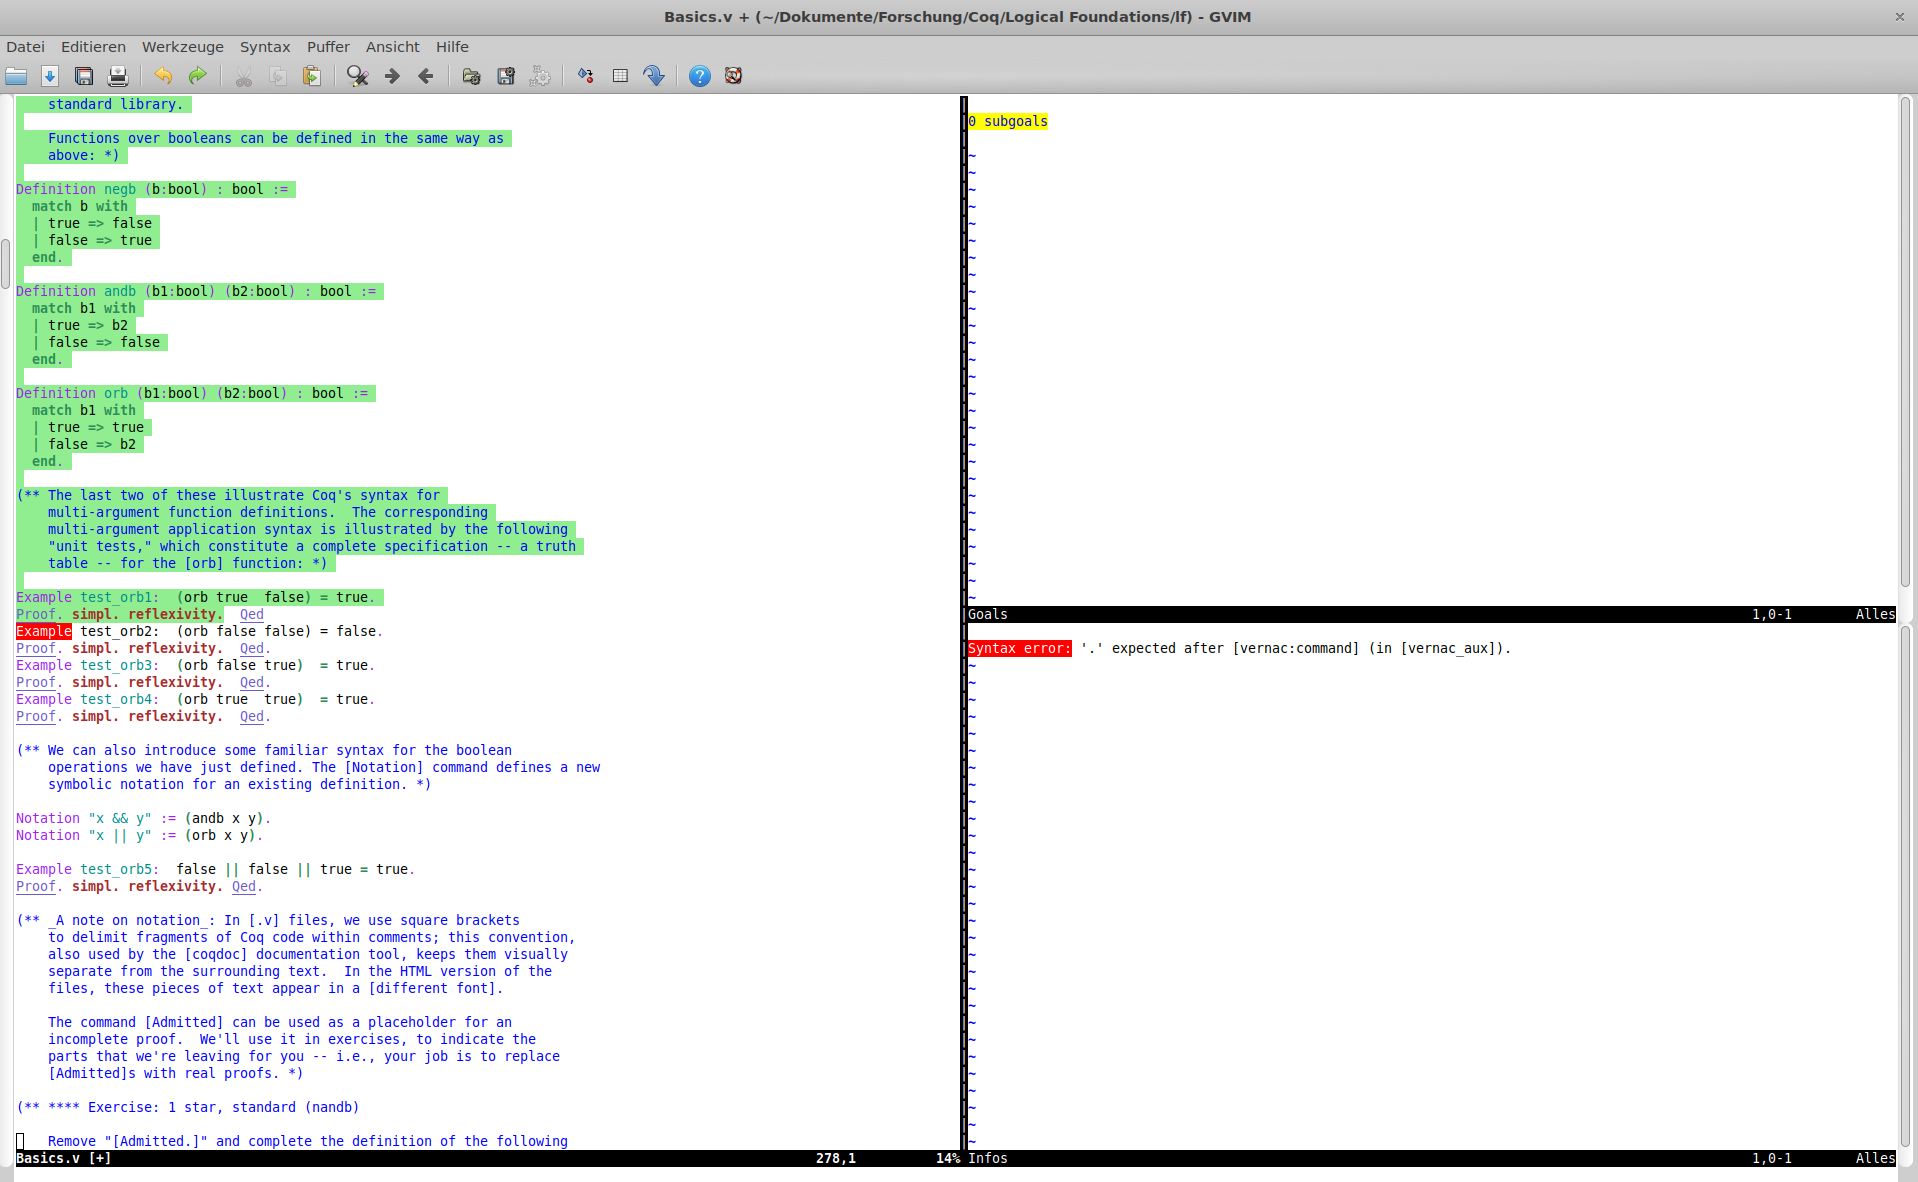
\includegraphics[width=0.9\textwidth]{CoqIDE.png}
\caption{Coq interface launched in gvim using coquille.\\ 
Left window: The open Coq-script \texttt{Basics.v}.
Upper right: The {\itshape goal window}. 
Lower right: The {\itshape message window}.}
\label{fig:Coquille}
\end{figure}

\subsection{Languages}
Coq uses three differnt languages. 
First, there is a vernucular language. 
It is a top-level interaction. 
It's keywords start with a capital letter e.g. \lstinline!Theorem!, \lstinline!Proof! and  \lstinline!Qed!. 
There is the tactics language (e.g. \lstinline!intros! and \lstinline!exact!).
And finally there is an unnamed language of Coq-terms. 
It consits of a lot of operators (e.g. \lstinline!for all A:Prop, A -> A!).
Technically, it is part of the tactics language, but it is useful to think of it as it's own thing.

\cleardoublepage

% Kapitel mit Inhalt

\cleardoublepage

\section{Basic Functional Programming in Coq}



\subsection{Introduction}

In this chapter we are going to introduce the most essential elements of Coq's functional programming language called {\itshape  Gallina}. 
Moreover, {\itshape tactics}, which can be applied to prove properties of Coq programs, are introduced.


\subsection{Data and Functions}

 \paragraph{Enumerated Type}
 
  The built-in features set in Coq is extremely small. In particular, Coq is a powerful mechanism for defining data types from scratch.
  Current Coq distributions come preloaded with an extensive standard library.
  Boolean, numbers, data struts like lists and hash tables.\\
  In this course we are going to explicitly recapitulate the used definitions.
   
  
  \begin{example}
  We are defining a type called \lstinline!day!.
  \begin{lstlisting}
    Inductive day: Type :=
	  | monday
	  | tuesday
	  | wednesday
	  | thursday
	  | friday.
	  | saturday.
	  | sunday.
	  \end{lstlisting} 
  
  The type members are called \lstinline!monday!, \lstinline!tuesday! , \lstinline!wednesday! \ldots{} and \lstinline!sunday!.\\
  
  We are defining a function operating on \lstinline!day!: 
  \begin{lstlisting}
  Definition next_weekday(d:day) day:=
    match d with 
	  | monday => tuesday
	  | tuesday => wednesday
	  | wednesday => thursday
	  | thursday => friday
	  | friday => monday
	  | saturday => monday
	  | sunday => monday.
    end.  
  \end{lstlisting}
  \end{example}

  Coq is able of {\itshape type  interference}, whenever the type is not defined explicitly.
  But for readability, we are including types in the following.
   
  For testing the above definition and function we have three possibilities in Coq:
     
   \begin{enumerate}
   \item Compute a compound expression including the function:\\
 		 \lstinline! compute (next_weekday friday).  (* = monday : day *)! or \\
   		 \lstinline! compute (next_weekday (next_weekday saturday)). (* = tuesday : day *)!
   \item Record an expected behaviour as a Coq-\lstinline!Example! and verify the assertion: 
         E.g.: {\itshape The second weekday after Saturday is Tuesday.}  
   
		   \begin{lstlisting}
		   		Example. test_next_weekday: (next_weekday (next_weeekday(saturday)) = tuesday 
		   		proof. simpl. reflexivity. Qed.
		   \end{lstlisting}
   			The details of the implementation are not important right now. We are going to come back to them later.
   \end{enumerate}   

    Moreover, Coq can be asked to \lstinline!extract! a program from our \lstinline! Definition! in a programming language, which is more conventional, being equipped with a high performance compiler.
    In particular this is one of the main uses of Coq. 
    It provides a method to transfer proved-correct algorithms in Gallina to efficient machine code.
    (Assuming the correctness of the corresponding high performance compile e.g. the Ocaml, Haskell or Scheme compiler. 


\subsection{Booleans}

    Of course, Coq provides an default implementation of Booleans.
    (See the \href{https://www.cs.princeton.edu/courses/archive/fall07/cos595/stdlib/html/Coq.Init.Datatypes.html}{Coq.Init.Datatypes in the Coq-Library documentation}).  
    In the following we are going to be consistent with the Coq library documentation according to the standard library.
    We are going to introduce coinciding selfdefined data types whenever possible.
    Booleans can be defined as follows:
    
    \label{Def:booleans}
    \begin{lstlisting}    
    Inductive bool: Type :=
      | true
      | false.
    \end{lstlisting}
    
    A function with multiple input arguments is implemented by
    \begin{lstlisting}
    Definition orb (b1: bool) (b2: bool) : bool :=
    match b1 with
	  | true -> true
	  | false -> b2
    end.
    \end{lstlisting}
    
    The functions \lstinline!negb! and \lstinline!andb! corresponding to the boolean functions {\emph negation} and {\emph and} are implemented in a similar manner.
     
    And a new symbolic notations is implemented as follows
    \begin{lstlisting}
    Notation "x && y" := (andb x y).
    Notation "x||y" := (orb x y).
    \end{lstlisting}
    
     
\subsection{Notation}
    As in the Coq doc documentation tool the following notation convention is introduced:
     
    \begin{enumerate}
     \item In \texttt{.v-files} comments are annotated by \lstinline!(* some comment *)!. 
     \item Within these comments Coq-code is denoted by \lstinline![example].! 
     \item And we write \lstinline! Admitted.! at the end of an incomplete proof.    
     \end{enumerate}
     
     
\subsection{Types}
     Every expression in Coq has a type.
     \begin{enumerate}
      \item  \lstinline* Check true.* gives the type of the expression \lstinline! boolean!.
      \item \lstinline! Check negb.! returns \lstinline! bool -> bool! . (Read as  ``bool arrow bool'').
              It is the functions input data type and the output data type, given input data of that type.
       \item \lstinline! andb! returns \lstinline!bool->bool->bool!. This function produces an output of type \lstinline! bool! given two inputs of type \lstinline! bool!.
     \end{enumerate}
   
\subsection{New Types from Old}
     
     
	 Note that so far the data-types we have seen were enumerated types.
	 Let's define a data type \lstinline!rgb! and a data type, whose constructor takes this type as an argument.
	\begin{lstlisting}
	 Inductive rgb: Type:=
	  | red     (* These are *)
	  | green   (* the expressions *)
	  | blue.   (* in the set [rgb]. *)
	 \end{lstlisting}
	 The constructors of the type \lstinline!rgb! are \lstinline!red, green! and \lstinline!blue!. 
	 
	 \begin{lstlisting}
	 Inductive color: Type := 
	  | black
	  | white
	  | primary (p:rgb). (* If [p] is in the set [rgb], then the constructor [primary] applied to the argument [p] is an expression in the set color.*) 
	 \end{lstlisting}
	 
	 The expressions in the set color are \lstinline!black, white! and \lstinline!primary!.
	 Note that, expressions formed as above are the only ones belonging to the sets \lstinline!rgb! and \lstinline!color!.
	 

\subsection{Tuples}

    A single constructor with multiple parameters can be used to create a type \lstinline! tuple!.
	\begin{example}[A nybble: half a byte]~\\\vspace{-10mm}
 	 	\begin{lstlisting}
 	 		Inductive bit: Type := (*a bit*) 
 	 		 |B0
 	 		 |B1.
 		    Inductive nybble: Type := (*a nybble*)
 		   	 |bits( b0 b1 b2 b3: bit).
 		   			 	
 		   	Check(bits B1 B0 B1 B0) (* => bits B1 B0 B1 B0 : nybble *)
 		\end{lstlisting}
 		Hence, a tuple of four bits is a nybble.
 		
 		Assume we would like to test a nybble in order to see if all its bits are 0. We are unwrapping the nybble by pattern-matching:
 		\begin{lstlisting}
 		Definition all_zero(nb: nybble): bool :=
 		  match nb with
 	  	    |(bits B0 B0 B0 B0) -> true
 		    |(bits _ _ _ _) -> false (* This wildcard pattern was included to avoid inventing variable names, which are not going to be used. *) 
 		  end.
 		 \end{lstlisting}
 	\end{example}
 	

\subsection{Modules}

	Coq provides a {\itshape module system} to aid organizing large developments.
	In this course most of it is not going to be needed.

	\begin{lstlisting}
	Module X 
	...
	End X
	\end{lstlisting}

\subsection{Numbers}

  Note that on the one hand the types day, bool, bits and tuples have a finite set of values, while on the other hand the set of natural numbers $\mathbb{N}$ is an infinite set.
 
  Hence, we have to construct $\mathbb{N}$ using a data type with a final number of constructors. 
  Recall, many representations of $\mathbb{N}$ exits (e.g. hexadecimal with base 16, octa with base 8, binary with base 2).
  The most familiar might be the decimal representation.\\
  However, each representation of $\mathbb{N}$ can be useful under different circumstances. 
  The binary representation is valuable in computer hardware, because it presents a simple circuitry.
  Here we are aiming to make proofs simple using the unary (base 1) representation.
  
  \begin{lstlisting}
  Module NatPlayground
  Inductive nat: Type :=
    | 0
    | S (n:nat).
  \end{lstlisting}
  
  One might picture this representation by scratches on a wall in prison. \\
  It uses two constructors: 
  \begin{itemize}
  \item The letter \lstinline!0! represents the natural number zero. 
  \item The letter \lstinline!S! represents a natural number $n\in\mathbb{N}\setminus\{ 0\}$.  
  \end{itemize}
  There is a way of converting this representation refereed to as \lstinline!nat! into its decimal representation. This is elaborated as follows.
  \begin{example}
  
	  \begin{tabular} {r l}
	  
		  \texttt{unitary}				& \texttt{decimal}	\\
		  \texttt{\lstinline!0!} 		&: 0 				\\
		  \texttt{\lstinline! S 0!}  	&: 1				\\
		  \texttt{\lstinline! S ( S 0)!}	&: 2				\\
		  \texttt{\lstinline! S( S ( S 0))!}	&: 3				\\
		    
	  \end{tabular}
  \end{example}
  Moreover, it is easy to see the following: 
  \begin{itemize}
  \item The expression \lstinline! 0! belongs to the set \lstinline! nat!.
  \item If \lstinline! n ! is in the set \lstinline! nat!, it follows \lstinline! S n ! is an expression belonging to the set \lstinline! nat !.
  \item And expressions belong the set \lstinline! nat! if and only if they are  formed by either of those methods (i.e. \lstinline! 0 ! or  \lstinline! S n!). 
  \end{itemize}
  
  
  Note that the same results apply to the definitions of \lstinline! day!, \lstinline! bool! and \lstinline! color!.
  These conditions are a precise force of the \lstinline! Inductive! declaration. 
  Expressions adult from other data constructors like \lstinline!true!, \lstinline! false!, \lstinline!andb(S(false( 0 ( 0 S ))))! do not belong to this set.  
  But on the other hand, \lstinline!0! and \lstinline!S! are arbitrary symbols chosen in the defined representation. 
  Actually the {\itshape interpretation} of these marks is given by their usage in computing.
  To realize this functions, which ``pattern match'' a representation of natural numbers, are written.
  
  We are following the idea:  If n has the form \lstinline! Sn'! for some \lstinline! n'! in the set \lstinline!nat!, then return  \lstinline! n'!.
  \begin{example}[predecessor function]~\\\vspace{-10mm}
   \begin{lstlisting}
  	 Definition pred (n:nat): nat :=
   		match n with 
   	     | 0 => 0
   	     | S n' => n'
   	    end. 
   	  
   	 End NatPlayground
   	 
   	 check( S(S(S(S(0)))). (* = 4: nat *)
   \end{lstlisting}
  \end{example}
  Because natural numbers are such a pervasive form of data, Coq always prints out a natural number as decimal by default.
  (It uses a tiny `` bulid-in magic'' for paring and printing.)
 
  \begin{lstlisting}
  Definition minustwo( n: nat) : nat :=
    match n with
      | 0 =>  0
      | S 0 =>  0
      | S ( S n') = > n'
     end.
     
   Compute( minustwo(4)) (* = 2: nat *)
  \end{lstlisting}  
  Sofar we have seen the functions \lstinline!S!, \lstinline!pred! and \lstinline!minustwo!.
  Note that, there is a fundamental difference.
  The functions \lstinline!pred! and \lstinline!minustwo! apply computaional rules. 
  There are no computaional rules about \lstinline!S!.
  I.e., by the definition of \lstinline!pred!, \lstinline!pred 2! can be simplified to \lstinline!1!. 
  In the case of \lstinline!S! no such behavior exists.
  The definition of \lstinline!S! has no bahavior at all.\\ 
    
  In order to define more functions over numbers pattern matching is not sufficient. We are introducing recursion.
  Recursion in Coq is notated by the keyword \lstinline!Fixpoint!.
  
  \begin{lstlisting}
  Fixpoint evenb (n:nat) : bool :=
  	match n with
  	| 0 => true
  	| S 0 => false
  	| S (S n') => evenb n'
  	end.
  	
  	Definition oddb (n:nat): bool := negb (even bn). (* a simple definition of odd *)
  	
  	Example test_oddb1: oddb1 = true
    	Proof. simpl. reflexivity. Qed.
  \end{lstlisting}
   Note that in this proof \lstinline!simpl.! actually has no effect on the goal. 
   All the work is done by \lstinline!refelxivity!. 
   We are going to come to back to that later.
   
   \subsection{Multi Argument-Function by Recursion}
   
   \begin{lstlisting}
   Module NatPlayground2.
   
   Fixpoint plus (n : nat) (m : nat): nat :=
     match n with
       | 0 => m
       | S n' => S (plus n' m)
     end.
     
    Compute (plus 3 2). 
   \end{lstlisting}
   
    A notation convention for calling functions or matching two expressions for multiple arguments of the same type exist in Coq, too.
   
   \begin{lstlisting}[label = lst:minus_nat, caption={ \lstinline!minus! and \lstinline!exp!}]
    Fixpoint minus (n m: nat): nat :=
     match n, m with
       | 0 , _ => 0
       | S _ , 0 => n
       | S n', S m' => minus n' m'
      end.
      
     Example test_mult1: (minus 3 2) = 1.
     
      
     End NatPlayground2
     
     Fixpoint exp (base power : nat) : nat :=
       match power with
         | 0 => S 0
         | S p => mult base (exp base p)
       end.
         
   \end{lstlisting}
        
   \subsection{Introducing Notations}


    For the Coq-parsers and Coq-prettifyers sake we are introducing a new notation:
    
    \begin{lstlisting}
     Notation " x + y ":= (plus x y)
                      (at level 50, left associativity) (*This line is not of interest for our purpose.*)
                      : nat_scope. (*This line is not of our interest.*)
                      
     Check(( 0 + 1 ) + 1).
    \end{lstlisting} 
   
   And these are some more functions defined for our purpose. 
   The intersterd reader is referend to the literature for an exact definition.  
   
   \begin{center}
   \begin{tabular}{|c|c|c|c|}
     \hline 
 	  notation      & function        & functionality                       & uses           \\  \hline
 	  x - y         & minus           & subtract two natural numbers       & see listing  \ref{lst:minus_nat} \\  \hline
      x * y         & mult            & multiply natural numbers            & nested matches \\  \hline   
   	  x =? y        & eqb             & test natural numbers                & nested matches \\  
  	                &                 & for equality yielding a boolean     &                \\  \hline
   	  x <=? y       & leb             & test if a first argument            & nested matches \\  
   	                &                 & is less or equal yielding a boolean &                \\  \hline
   \end{tabular}
   \end{center}
	Note that we when we sayed that Coq comes with almost nothing built-it in, we really mean it.
    Even equality testing is a user-defined operation.
    
    
        
   \subsection{Proof by Simplification}
   
   
   Till now we have defined a few data types and functions.
   Example: We have seen all claims were shown by the same proofs. \lstinline!simple! and \lstinline!refelctivity!. 
   \lstinline!simple! simplified equations and \lstinline!reflexivity! checked weather both sides contain identical values.
   An on the hand rule might say that, \lstinline!simple! can be used to show more simple properties.
   For example we consider the following observation: ``0+n reduces to n, no matter, what n is.''
   The mathematical precisely formulated statement can be proven by the definition of zero directly.
   
   \begin{example}
	   \begin{theorem}
  	   \begin{lstlisting}
   		Theorem. plus_0_n: for all n: nat, 0+n = n.
   		  Proof. intros n. simpl. refelxivity. Qed.
    	\end{lstlisting}	
	\end{theorem}
	\end{example}              
    \begin{remark}
    	Reflexivity does not only check weather both sides of an equation contain identical values. 
    	On top of that it simplifies, which makes it more powerful. 
    	We have seen \lstinline!simpl! added in our examples so we can see the intermediate state.
    	Therefore, the above proof can be simplified by omitting \lstinline!simpl!. 
     \end{remark}


	\begin{lstlisting}
    Theorem plus_0_n': for all n: nat, 0 + n = n.
    Proof: intros n. reflexivity. Qed.	
    \end{lstlisting}
    
    By looking at the Coq output we can see that \lstinline!reflexivity! somehow tries ``	unfolding'' defined terms.
    
    Note that \lstinline!example! and \lstinline!theorem! (and \lstinline!Lemma!, \lstinline!Fact!, \lstinline!Remark! and a few other),
    mean pretty much the same in Coq, while in Mathematics they do not.
    
   
     
    \paragraph{Prooftechniques}
    
    \paragraph{Intros, Simplification and Reflexivity}
     Whenever a \lstinline!Theorem! starts with \lstinline!for all n!, we might start a proof by the phrase:
     Assume \lstinline!n! is some natural number. By \lstinline! intros n! we can tell this to Coq.\\
     A {\itshape tactic} is a command used between \lstinline!proof! and \lstinline! Qed.!, 
     which guides the process of checking some claim for example the keyword \lstinline! intros!, \lstinline! simpl! and \lstinline!reflexivity.! 
     are tactics.
     \paragraph{Notation} 
     The suffix \lstinline!_|! is pronounced ``on the left''. 
     \begin{example}
	     \begin{lstlisting}
	      Theorem mult_0_l: for all n: nat, or n = 0.
	        proof: intros n. refelexivity. Qed.
	     \end{lstlisting}
     \end{example} 
  
   Let's recall what reflexivity in terms of an equivalence relation means.  
   \begin{definition}[Equivalence Relation]
   Assume $x,y\in \mathcal{M}$ an arbitrary set $\mathcal{M}\neq\emptyset$ and $\thicksim\subset A \times A $ an arbitrary relation.
   Then $\thicksim$ is sayed to be an equivalence relation if and only if:
   \begin{enumerate}
   \item $a\thicksim a$ (reflexivity)
   \item $a \thicksim b$ if and only if $b \thicksim c$ (symmetry)
   \item if $a \thicksim b$ and $ b\thicksim c$ then $a \thicksim c$ (transitivity) 
   \end{enumerate}
   \end{definition}
     
   Due to the \href{https://pjreddie.com/coq-tactics/}{Coq tactics index} it is recommended to use reflexivity, if your goal is to prove that something is equals to itself.  
      
     \paragraph{Proof by Rewriting}
     
     Consider the following example theorem:     
     %\begin{example}\\
	 \begin{lstlisting}[caption=Example]
	 Theorem plus_id_examples: for all n m: nat
       n = m -> 
	   n+n = m+m.	 
	 \end{lstlisting}  
	 %\end{example}   
	
	 We would like to show this theorem instead by making a claim about all numbers by looking at the special case when \lstinline!n=m!.
     \lstinline!->! corresponds to the mathematical implication operator $\implies$. 
     
%     The {\itshape tactic} \lstinline! intros!.     
    
    
     Note that, the arrow \lstinline!->! tells Coq to rewrite the object of focus from left to right and \lstinline!<-! can be used to rewrite from right to left.
     
     \begin{tabular} {|l|l|l|}
     	\hline
     	  command                        & a mathematical translation          & comment \\  \hline
     	 \lstinline!proof.!              & $\text{wts}: \forall m,n \in \mathbb{N}:$ & Moves the last used \\   
     	      	                         &  $n = m \implies n+n = m+m \qquad$  &         \\     
     	      	                         &  $Proof:$                           & theorem into the focus.\\  
       	                                 &                                     &                                    \\   \hline
         \lstinline!  intros n m.!       & Assume $m,n \in \mathbb{N}.$        & Moves the universally quantified variables\\
                                         &                                     & n and m into the focus.   \\   \hline                                            
          \lstinline!  intros H.!        & $H :=\{n=m\}$                       & Moves the hypothesis into              \\ 
    	                                 &                                     & the focus of Coq.                                          \\    \hline   
     	 \lstinline!  rewrite -> H.!     &                                     & Replace by H from left to right and                            \\  
     	                                 & $H \wedge n:=m$ $\implies m+m = m+m$& rewrite the goal using the hypothesis.           \\ \hline
     	 \lstinline!  reflexivity.!      & trivial                             &  We obtained a trivial statement.                 \\ \hline
    	 \lstinline! Qed.!                & Qed.                                &  Quod era demonstrandum.                         \\  \hline
    	 
     \end{tabular}
   
   
   
   
   We can also use \lstinline!rewrite! with a previously proved theorem instead of a hypothesis of context.
   If the statement of the previously proved theorem involves prequantified variables, Coq reuses them.
   
   \begin{lstlisting}
   Theorem mult_0_plus: for all n m: nat,
   (0 + n) * m = n * m.
   Proof.
     intros n m.                   (* Let $n,m\in\mathbb{N}$ *) 
     refelxivity -> plus_0_n.       (* rewrite $0+n$, by n *)
     reflexivity.                  (* m = m *)
     Qed.
   \end{lstlisting}   

	\paragraph{Admitted and Abort}
	
	The command \lstinline!Admitted! tells Coq to skip a proof of a theorem and to accept it as given.
	It can be used in long proofs to subsidiary state longer \lstinline!Lemmas!.
	If a proof was started it can be interrupted by the command \lstinline!Abort!.
	Note, if a proof was forgotten in the following nonsense is a able to be shown. \\
	
	
 \subsection{Proof by Case Analysis}
   Consider the following example. It clearly demonstrates that, it is not possible to prove everything using the simplification tactic.   
   
   
   \paragraph{Destruct}	
   \begin{lstlisting}
   Theorem plus_1_neq_0_firsttry : for all n : nat,
     (n + 1) =? 0 = false.
     Proof.
     intros n.
     simpl. (* does nothing! *)
   Abort.
   \end{lstlisting}
	Write something short from the book, why it obviously is not going to work.\\
	
	Note that if \lstinline!n=0! it can be calculated that \lstinline!n+1=?0! and set it equals to  \lstinline!false!. 
	And if \lstinline!n=Sn'! for some \lstinline!n'! we can not calculate the expression.
	Although we don't know, which number \lstinline!n+1! is, we can calculate that it begins with an \lstinline!S!.
	It follows \lstinline!n+1= ? 0! yields \lstinline!false!.
	
    Hence we would like to generate two subgoals including variables named as in the called \lstinline! intros! pattern.	   
        
    Therefore we are using the tactics \lstinline! destruct!	
	\begin{lstlisting}
	intros n.
	destruct n as[ |n'] eqn: E
	\end{lstlisting}
	
	\begin{enumerate}
		\item 	The expression \lstinline![.. ]! is called the intro pattern. It is a list of lists of names separated by \lstinline!|!.
		\item   Any data type can be referd to in the into pattern's list.
		\item In this case the first entry of our list is empty, because the \lstinline!0!-constructor is nullary and the constructor of \lstinline!S! is unary, therefor it is written \lstinline!n'! as the second member of our list.
		\item \lstinline!E! is the variable for the equation in the following
		\item In general every subgoal, which follows the destruct is going to be marked by \lstinline!-!.
	\end{enumerate} 
	
	The bullets are not necessarily to list sufficiently. 
	Coq asks to show every listed subgoal in sequence.
	But due to readability and clearance, ensurence of correctness and convenience in debugging sub goals should be listed.
	
	Moreover, there are no hard or fast rules in proof formatting (i.e. indents and linebreaks). 
	Bullets in the beginning of the line foster readability and maximally 80 characters per line are convenient.
	
	\begin{example}
	  \begin{lstlisting}
	  	Theorem newb_involutive: for all b: bool,
	  	  neg b ( neg b ) = b.
	  	  
	  	Proof. 
	  	  intros b destruct b eq n: E
	  	    - reflexivity. 
	  	    - reflexivity. 
	  	   Qed.  
	  \end{lstlisting}
	\end{example}
	 
	 
	
	

   
\section{Importing}


In order to use the definitions from the previous chapter we are going to compile the file 
\texttt{Basics.v} and import the compiles version in the current file \texttt{Induction.v}.
(In case the book \cite{PACGGHSY} is used and downloaded as an archive, the following steps can be skipped.)   

\subsection{Building Coq Libraries}

First of all, a Coq project, called {\itshape \_CoqProject}, is created.  
It is going to map the current directory ``\texttt{.}'' to the directory \texttt{lf} wherein the source files are kept.
Using the CoqIDE, Proof General or executing Coq via the command line the compiling and building process differs.
The Proof General using reader is refereed to the literature \cite[Section, Induction, Proof by Induction]{PACGGHSY}.\\

Create a file called \texttt{\_coqProject} within the working directory which contains the file \texttt{Basics.v}.
Within this file add the line 

\begin{lstlisting}[caption = \lstinline!naming a library!]
-Q .LF
\end{lstlisting}

which declares the library's name \texttt{LF.Basics}. 
To make the executable \texttt{Basics.vo}-file out of the \texttt{Basics.v} multiple options exist.

Using the CoqIDE, the file \texttt{Basics.v} should be opened, and the button in the compile menu  ``{\itshape Compile Buffer}'' is clicked.
If using the command line the file \texttt{Basics.vo} can be build or compiled using the Coq  make-file utility.
By the way, the {\itshape Coq-makefile utility } is installed together with Coq.
Type the following console-command:
\begin{lstlisting}[language=bash, caption = \lstinline!coq-makefile!, label = lst:coq-makefile]
coq_makefile -f _CoqProject *.v -o Makefile
\end{lstlisting}

In addition run this command, whenever files to the working directory \texttt{lf} were added or removed.
To compile \texttt{Basics.v}, call either on of the following commands 
\begin{lstlisting}[language=bash, caption = \lstinline!make!, label = lst:make]
make (* builds the complete directory *)
make Basics.vo (* builds Basics.vo *)
\end{lstlisting}
Note that, \lstinline!make! compiles and calculates dependencies automatically. 
The Coq-compiler, which is called {\itshape coqc} can be called by: 
\begin{lstlisting}[language=bash, caption =\lstinline!coqc!, label = lst:coqc]
coqc -Q.LF Basics.v
\end{lstlisting}
But remember always to prefer \texttt{make} over compiling, because of the dependencies.\\
 
To include the compiled chapter \texttt{Basics.vo} into the source code of the chapter \texttt{Induction.v} it is written
\begin{lstlisting}[language = bash, caption = \lstinline!Require Export!, label = lst:RequireExport]
From LF Require Export Basics.
\end{lstlisting}
into the first line of the \texttt{Induction.v}-file.

 

\subsection{Potential Troubles}

If an error arises which complains about missing identifiers in the file the "load path" for Coq might not be set up correctly.
Checking the loaded path by the command
\begin{lstlisting}[language = bash, caption = checking the loaded path, label = lst:PrintLoadPath]
Print LoadPath.  
\end{lstlisting} 
might be helpful. The error message
\begin{lstlisting}[language = bash, caption = possible  version error, label = lst:possibleVersionError ]
  Compiled library Foo makes inconsistent assumptions over library Bar
\end{lstlisting}
might be generated, because incompatible versions of Coq are installed on a machine.
In particular,  CoqIDE and Proof General can use different versions of Coq for compiling. 

To resolve these issues build the files again.\\

Receiving the error message 
\begin{lstlisting}[language = bash, caption= possible compiling error, label=lst:PossibleCompilingError]
Unable to locate library Basics.
\end{lstlisting}
might be caused if two libraries are dependent and \texttt{Bar} was modified and compiled singly.
To overcome this issue, build \texttt{Basics.vo} again.
In case to many files are affected build everything again.
\begin{lstlisting}[language=bash, caption = rebuilding libraries, label = lst:RebuildingLibraries]
Make clean, make
\end{lstlisting}

Using the CoqIDE and running \texttt{coqc} in the command line might cause inconsistency. 
A workaround of this issue is always using the {\itshape make} button from the CoqIDE and never calling the compiler directly.

\section{Induction}

\subsection{Proof by Induction}
In the proof \ref{lst:plus0nPrime} it was shown have , 
that \lstinline!0! is the neutral element from the left if the natural numbers \lstinline!nat! is studiet as a group. 

Is should be shown that zero is is the natural element from the right:
\begin{lstlisting}
Theorem plus_n_0_first: for all n: nat
  n = n + 0.  
\end{lstlisting}

But the tactics, which were introduced till know, are not sufficiently powerful to proof this theorem.

\begin{lstlisting}
Theorem plus_n_O_firsttry : forall n:nat,
  n = n + 0.
\end{lstlisting}

Applying refelxivity can not proof the theorem. In fact, simplifying the expression \lstinline!n + 0 !, leads to nowhere.
Because looking at the definition of \lstinline!plus!, it is obvious.
If \lstinline!n! is an unknown number, the  \lstinline!match! can not be applied.
  
\begin{lstlisting}
Proof.
  intros n.
  simpl. (* Does nothing. *)
Abort.
\end{lstlisting}

Proofing by the \lstinline!destruct!-tactic is going to fail, because in the case \lstinline!n = Sn'! the expression \lstinline!S n' = S n' + 0! can not be simplified by the same reason as above.
\begin{lstlisting}
Proof.
  intros n. destruct n as [| n'] eqn:E.
  - (* n = 0 *)
    reflexivity. 
  - (* n = S n' *)
    simpl.       (*Does nothing.*)
Abort.
\end{lstlisting}

Recall the mathematical principle of induction.
Due to apply induction in Coq the steps are the same and the syntax is simialar to the \lstinline!destruct! tactics.
 

\begin{lstlisting}
Theorem minus_diag : forall n,
  minus n n = 0.
Proof.
  intros n. induction n as [| n' IHn'].
  - (*case: n = 0 *)
    simpl. reflexivity.
  - (*case: n = S n' *)
    simpl. rewrite -> IHn'. reflexivity.  
  Qed.
\end{lstlisting}

The \lstinline!as!-clause has two parts seperated by \lstinline!|!.
\begin{itemize}
	\item In the above statement of \lstinline!induction! the first subgoal is to show the induction basis for \lstinline!n =0!.
	\item And the second subgoal is the induction step for \lstinline!n = Sn'!, since \lstinline!nat! is defined inductivly (see listing  \ref{lst:DefNat}).
	      The assumption \lstinline!n'+0 = n'! is added to Coq's context named as \lstinline!IHn'! as induction hypothesis.
		  It must be shown \lstinline! Sn' = Sn' +0!. \
          Applying \lstinline!simpl.! yields \lstinline!Sn' = S(n'+0)!, which follows from the induction hypothesis. 
          Hence, \lstinline!relfexivity.! finishes this proof.
\end{itemize} 






%Kapitel ohne Inhalt
\section{To Answer}

Add how does the proof tactic \lstinline!reflexivity! actually work \label{sec:reflexivity} (see \ref{subsec:proof-techniques})

Steffen's interest

The solutuin is here: \cite{ExtractingProgrammsinOCAMlandHaskell}

Can a code generator be build e.g. Ada VHDh, Scala? See sec. \ref{subSec:DataAndFuctions} bullet \ref{CoqAsCodeGen}.


%%%%%%%%%%%%%%%%%%%%% content end %%%%%%%%%%%%%%%%%%%%%%%%%%%%%%%%%

\begin{center}
\mbox{}
\vfill
$\star \star \star$ \textsc{Ende} $\star \star \star$
\end{center}

% Appendix
%%%%%%%%%%%%%%%%%%% lecture notes mbasics %%%%%%%%%%%%%%%%%%%%%%%%%%

\cleardoublepage
\appendix


%% include this later
%% Mengen, Relationen und Funktionen
\section{Grundlagen und Schreibweisen}

\subsection{Mengen}Es ist sehr schwer den fundamentalen Begriff der Menge mathematisch exakt
zu definieren. Aus diesem Grund soll uns hier die von Cantor im Jahr $1895$ gegebene
Erklärung genügen, da sie für unsere Zwecke völlig ausreichend ist:

\begin{definition}[Georg Cantor (\cite{Ca85})]
Unter einer ,\dindex{Menge}' verstehen wir jede Zusammenfassung $M$ von 
bestimmten wohlunterschiedenen Objecten $m$ unsrer Anschauung oder 
unseres Denkens (welche die ,\dindex{Elemente}' von $M$ genannt werden) zu 
einem Ganzen\footnote{Diese Zitat entspricht der originalen
Schreibweise von Cantor.}. 
\end{definition}

\noindent Für die Formulierung "`genau dann wenn"' verwenden wir im Folgenden
die Abkürzung \gdw\index{gdw=gdw.} um Schreibarbeit zu sparen.

\subsubsection{Die Elementbeziehung und die Enthaltenseinsrelation}
Sehr oft werden einfache große lateinische Buchstaben wie $N$, $M$, $A$, $B$ oder $C$ 
als Symbole für Mengen verwendet und kleine Buchstaben für die Elemente einer Menge.
Mengen von Mengen notiert man gerne mit kalligraphischen Buchstaben wie $\mathcal{A}$, 
$\mathcal{B}$ oder $\mathcal{M}$.
\begin{definition}
\label{InclSet}
Sei $M$ eine beliebige Menge, dann ist
\begin{itemize}
%
\item $a \in M$ \gdw\ $a$ ist ein Element der Menge
$M$\index{$\in$},
%
\item $a \not\in M$ \gdw\ $a$ ist kein Element der Menge $M$\index{$\not\in$},
%
\item $M \subseteq N$ \gdw\ aus $a \in M$ folgt $a \in N$ ($M$ ist
\dindex{Teilmenge}\index{Menge!Teil-} von $N$)\index{$\subseteq$},
%
\item $M \not\subseteq N$ \gdw\ es gilt nicht $M \subseteq
N$. Gleichwertig: es gibt ein $a \in M$ mit $a \not\in N$ ($M$ ist
keine Teilmenge von $N$)\index{$\not\subseteq$} und
%
\item $M \subset N$ \gdw\ es gilt $M \subseteq N$ und $M \not= N$ ($M$ ist
echte Teilmenge von $N$)\index{$\subset$}.
%
\end{itemize}
Statt $a \in M$ schreibt man auch $M \ni a$\index{$\ni$}, was in
einigen Fällen zu einer deutlichen Vereinfachung der Notation führt.
\end{definition}

\subsubsection{Definition spezieller Mengen}
\label{MengenDef}
Spezielle Mengen können auf verschiedene Art und Weise definiert
werden, wie z.B.
\begin{itemize}
%
\item durch Angabe von Elementen:\ So ist $\set{\enu{a}{1}{n}}$ die Menge,
die aus den Elementen $\enu{a}{1}{n}$ besteht, oder
%
\item durch eine Eigenschaft $E$:\ Dabei ist $\set{a \mid E(a)}$ die Menge
aller Elemente $a$, die die Eigenschaft\footnote{Die Eigenschaft $E$
kann man dann auch als \dindex{Prädikat} bezeichnen.} $E$ besitzen.
%
\end{itemize}
Alternativ zu der Schreibweise $\set{a \mid E(a)}$ wird auch oft 
$\set{a \colon E(a)}$ verwendet.

\goodbreak
\begin{example}
\label{ex:numbers}
Mengen, die durch die Angabe von Elementen definiert sind:
\begin{itemize}
%
\item $\mathbb{B} \eqd \set{0,1}$
%
\item $\N \eqd \set{0, 1, 2, 3, 4, 5, 6, 7, 8, \dots}$ (Menge der \dindex{natürlichen Zahlen}\index{Zahlen!natürlich})\index{$\N$}
%
\item $\Z \eqd \set{\dots, -4, -3, -2, -1, 0, 1, 2, 3, 4, \dots}$ (Menge der \dindex{ganzen Zahlen}\index{Zahlen!ganz})\index{$\Z$}
%
\item $2\Z \eqd \set{0, \pm 2, \pm 4, \pm 6, \pm 8, \dots}$ (Menge der geraden ganzen Zahlen)\index{$2\Z$}
%
\item $\PRIM \eqd \set{2, 3, 5, 7, 11, 13, 17, 19, \dots}$ (Menge der \dindex{Primzahlen})\index{$\PRIM$}
%
\end{itemize}
\end{example}

\begin{example}
Mengen, die durch eine Eigenschaft $E$ definiert sind:
\begin{itemize}
%
\item $\set{n \mid n \in \N \text{ und $n$ ist durch $3$ teilbar}}$
%
\item $\set{n \mid n \in \N \text{ und $n$ ist Primzahl und $n \le 40$}}$
%
\item $\emptyset \eqd \set{a \mid a \not= a}$ (die leere Menge)\index{$\emptyset$}
%
\end{itemize}
\end{example}

Aus Definition \ref{InclSet} ergibt sich, dass die leere Menge (Schreibweise: $\emptyset$) Teilmenge jeder Menge ist. Dabei ist zu beachten, dass 
$\set{\emptyset} \not= \emptyset$\index{$\set{\emptyset}$} gilt, denn $\set{\emptyset}$ 
enthält \emph{ein} Element (die leere Menge) und $\emptyset$ enthält \emph{kein} Element.

\subsubsection{Operationen auf Mengen}
\label{OpSetSect}

\begin{definition}
\label{OpSet}
Seien $A$ und $B$ beliebige Mengen, dann ist
\begin{itemize}
%
\item $A \cap B \eqd \set{a \mid a \in A \text{ und } a \in B}$
(\dindex{Schnitt}\index{Menge!Schnitt-} von $A$ und $B$)\index{$\cap$},
%
\item $A \cup B \eqd \set{a \mid a \in A \text{ oder } a \in B}$
(\dindex{Vereinigung}\index{Menge!Vereinigung-} von $A$ und $B$)\index{$\cup$},
%
\item $A \setminus B \eqd \set{a \mid a \in A \text{ und } a
\not\in B}$ (\dindex{Differenz}\index{Menge!Differenz-} von $A$ und $B$)\index{$\setminus$},
%
\item $\overline{A} \eqd M \setminus A$ (\dindex{Komplement}\index{Menge!Komplement-} von $A$ 
bezüglich einer festen Grundmenge $M$)\index{$\overline{A}$} und
%
\item $\PowerSet{A} \eqd \set{B \mid B \subseteq A}$ 
(\dindex{Potenzmenge}\index{Menge!Potenz-} von $A$)\index{$\PowerSet{A}$}.
%
\end{itemize}
Zwei Mengen $A$ und $B$ mit $A \cap B = \emptyset$ nennt
man \dindex{disjunkt}.

\begin{example}
Sei $A = \set{2, 3, 5, 7}$ und $B = \set{1, 2, 4 , 6}$, dann ist $A
\cap B = \set{2}$, $A \cup B = \set{1, 2, 3, 4, 5, 6, \allowbreak 7}$ und $A
\setminus B = \set{3, 5, 7}$. Wählen wir als Grundmenge die
natürlichen Zahlen, also $M = \N$, dann ist $\overline{A} = \set{n \in \N
\mid n \not= 2 \text{ und } n \not= 3 \text{ und } n
\not= 5 \text{ und } n \not= 7} = \set{1, 4, 6, 8, 9, 10, 11,
\dots}$. 

Als Potenzmenge der Menge $A$ ergibt sich die folgende Menge von Mengen
von natürlichen Zahlen $\PowerSet{A}
= \set{\emptyset,\allowbreak \set{2},\allowbreak \set{3},
\allowbreak \set{5},\allowbreak \set{7}, \allowbreak \set{2,3},
\set{2,5}, \allowbreak \set{2,7}, \allowbreak \set{3,5}, \allowbreak\set{3,7},
\allowbreak \set{5,7},\allowbreak \set{2,\allowbreak 3,5},\allowbreak
\set{2,3,7},\allowbreak \set{2,5,\allowbreak 7}, \allowbreak \set{3,\allowbreak 5,\allowbreak 7},\set{2,3,5,7}}$. 

Offensichtlich ist die Menge $\set{0,2,4,6,8, \dots }$ der geraden
natürlichen Zahlen und die Menge $\set{1,3,5,7,9, \dots }$ der
ungeraden natürlichen Zahlen disjunkt.
\end{example}
\end{definition}

\subsubsection{Gesetze für Mengenoperationen}
\label{SetOpSect}
Für die klassischen Mengenoperationen gelten die folgenden Beziehungen:
\begin{displaymath}
\begin{array}{rcll}
A \cap B &=& B \cap A & \text{Kommutativgesetz für den Schnitt}\\
A \cup B &=& B \cup A & \text{Kommutativgesetz für die Vereinigung}\\
A \cap (B \cap C) &=& (A \cap B) \cap C & \text{Assoziativgesetz für
den Schnitt}\\
A \cup (B \cup C) &=& (A \cup B) \cup C & \text{Assoziativgesetz für
die Vereinigung}\\
A \cap (B \cup C) &=& (A \cap B) \cup (A \cap C) & \text{Distributivgesetz}\\
A \cup (B \cap C) &=& (A \cup B) \cap (A \cup C) & \text{Distributivgesetz}\\
A \cap A &=& A & \text{Duplizitätsgesetz für den Schnitt}\\
A \cup A &=& A & \text{Duplizitätsgesetz für die Vereinigung}\\
A \cap (A \cup B) &=& A & \text{Absorptionsgesetz}\\
A \cup (A \cap B) &=& A & \text{Absorptionsgesetz}\\
\overline{A \cap B} &=& (\overline{A} \cup \overline{B}) &
\text{de-Morgansche Regel}\\
\overline{A \cup B} &=& (\overline{A} \cap \overline{B}) &
\text{de-Morgansche Regel}\\
\overline{\overline{A}} &=& A & \text{Gesetz des doppelten Komplements}
\end{array}
\end{displaymath}
Die "`de-Morganschen Regeln"' wurden nach dem englischen
Mathematiker \textsc{Augustus De Morgan}\footnote{\textborn $1806$ in
Madurai, Tamil Nadu, Indien - \textdied $1871$ in London, England}
benannt.

Als Abkürzung schreibt man statt $X_1 \cup X_2 \cup \dots \cup X_n$
(bzw.~$X_1 \cap X_2 \cap \dots \cap X_n$) einfach $\bigcup\limits_{i=1}^n X_i$
(bzw.~$\bigcap\limits_{i=1}^n X_i$). Möchte man alle Mengen $X_i$ mit
$i \in \N$ schneiden (bzw.~vereinigen), so schreibt man kurz
$\bigcap\limits_{i \in \N} X_i$ (bzw.~$\bigcup\limits_{i \in \N} X_i$).

\goodbreak

Oft benötigt man eine Verknüpfung von zwei Mengen, eine solche
Verknüpfung wird allgemein wie folgt definiert:

\begin{definition}["`Verknüpfung von Mengen"']
Seien $A$ und $B$ zwei Mengen und "`$\odot$"' eine beliebige
Verknüpfung zwischen den Elementen dieser Mengen, dann definieren wir
\begin{displaymath}
A \odot B \eqd \set{a \odot b \mid a \in A \text{ und } b \in B}.
\end{displaymath}
\end{definition}

\begin{example}
Die Menge $3\Z = \set{0, \pm 3, \pm 6, \pm 9, \dots}$ enthält alle
Vielfachen\footnote{Eigentlich müsste man statt $3\Z$ die Notation
$\set{3}\Z$ verwenden. Dies ist allerdings unüblich.} von $3$, damit
ist $3\Z + \set{1} = \set{1,\allowbreak 4,\allowbreak -2,\allowbreak
7,\allowbreak -5, 10, -8, \dots}$. Die Menge $3\Z + \set{1}$ schreibt
man kurz oft auch als $3\Z + 1$, wenn klar ist, was mit dieser
Abkürzung gemeint ist.
\end{example}

\subsubsection{Tupel (Vektoren) und das Kreuzprodukt}
Seien $A, A_1, \dots , A_n$ im folgenden Mengen, dann bezeichnet

\begin{itemize}
  % 
  \item $(\enu{a}{1}{n}) \eqd$ die Elemente $\enu{a}{1}{n}$ in genau dieser
  festgelegten \emph{Reihenfolge} und z.B.~$(3,2) \not= (2,3)$. Wir
  sprechen von einem $n$-Tupel\index{Tupel}\index{Tupel=$n$-Tupel}.
  % 
  \item $A_1 \times A_2 \times \dots \times
  A_n \eqd \set{(\enu{a}{1}{n}) \mid a_1 \in A_1, a_2 \in A_2, \dots
  ,a_n \in A_n }$ (Kreuzprodukt der Mengen $A_1, A_2, \dots ,
  A_n$)\index{Kreuzprodukt}\index{$\times$},
  %
  \item $A^n \eqd \underbrace{A \times A \times \dots \times
  A}_{n\text{-mal}}$ ($n$-faches Kreuzprodukt der Menge $A$)\index{$A^n$} und
  %
  \item speziell gilt $A^1 = \set{(a) \mid a \in A}$.
  %
\end{itemize}
Wir nennen $2$-Tupel auch \emph{Paare}\index{Paar}, $3$-Tupel
auch \dindex{Tripel}, $4$-Tupel auch \dindex{Quadrupel} und $5$-Tupel 
\dindex{Quintupel}. Bei $n$-Tupeln ist, im Gegensatz zu Mengen, eine 
Reihenfolge vorgegeben, d.h.~es gilt z.B.~immer $\set{a,b} = \set{b,a}$, aber 
im Allgemeinen $(a,b) \not= (b,a)$.

\begin{example}
Sei $A = \set{1, 2, 3}$ und $B = \set{a, b, c}$, dann bezeichnet das
Kreuzprodukt von $A$ und $B$ die Menge von Paaren $A \times B =
\set{(1,a), (1,b), (1,c), (2,a), (2,b), (2,c),\allowbreak (3,\allowbreak a), (3,b), (3,c)}$.
\end{example}

\subsubsection{Die Anzahl von Elementen in Mengen}
\label{cntSet}
Sei $A$ eine Menge, die endlich viele Elemente\footnote{Solche Mengen
werden als \dindex{endliche Mengen}\index{Menge!endliche} bezeichnet.}
enthält, dann ist
\begin{displaymath}
\cnt A \eqd \text{Anzahl der Elemente in der Menge $A$}.
\end{displaymath}
\noindent Beispielsweise ist $\cnt \set{4,7,9} = 3$. Mit dieser Definition gilt

\begin{itemize}
%
\item $\cnt(A^n) = (\cnt A)^n$\index{$\cnt$},
%
\item $\cnt \PowerSet{A} = 2^{\cnt A}$,
%
\item $\cnt A + \cnt B = \cnt(A \cup B) + \cnt (A \cap B)$ und
%
\item $\cnt A = \cnt (A \setminus B) + \cnt(A \cap B)$.
%
\end{itemize}

\subsection{Relationen und Funktionen}

\subsubsection{Eigenschaften von Relationen}
\label{PropRel}

Seien $\enu{A}{1}{n}$ beliebige Mengen, dann ist $R$ eine
\emph{$n$-stellige Relation}\index{Relation} \gdw 
\ $R \subseteq A_1 \times A_2 \times \dots \times A_n$. Eine
zweistellige Relation nennt man auch \dindex{binäre
Relation}\index{Relation!binär}. Oft werden auch Relationen
$R \subseteq A^n$ betrachtet, diese bezeichnet man dann als
$n$-stellige Relation über der Menge $A$.

\begin{definition}
Sei $R$ eine zweistellige Relation über $A$, dann ist $R$
\begin{itemize}
%
\item \dindex{reflexiv} \gdw \ $(a,a) \in R$ für alle $a \in A$,
%
\item \dindex{symmetrisch} \gdw \ aus $(a,b) \in R$ folgt $(b,a) \in R$,
%
\item \dindex{antisymmetrisch} \gdw \ aus $(a,b) \in R$ und $(b,a) \in R$ folgt $a =
b$,
%
\item \dindex{transitiv} \gdw \ aus $(a,b) \in R$ und $(b,c) \in R$ folgt $(a,c)
\in R$ und 
%
\item \dindex{linear} \gdw \ es gilt immer $(a,b) \in R$ oder $(b, a) \in R$.
%
\item Wir nennen $R$ eine \dindex{Halbordnung} \gdw $R$ ist reflexiv,
antisymmetrisch und transitiv,
%
\item eine \dindex{Ordnung} \gdw $R$ ist eine lineare Halbordnung und
%
\item eine \emph{Äquivalenzrelation}\index{Aquivalenzrelation=Äquivalenzrelation} 
\gdw $R$ reflexiv, transitiv und symmetrisch ist.
%
\end{itemize}
\end{definition}

\begin{example}
Die Teilmengenrelation "`$\subseteq$"' auf allen Teilmengen von $\Z$ ist
eine Halbordnung, aber keine Ordnung. 
\end{example}
\goodbreak

\begin{example}
Wir schreiben $a \equiv b \mod
n$, falls es eine ganze Zahl $q$ gibt, für die $a - b = q n$ gilt. Für $n \ge 2$
ist die Relation $R_n(a,b) \eqd \set{(a,b) \mid a \equiv b \mod n} \subseteq
\Z^2$ eine Äquivalenzrelation.
\end{example}

\subsubsection{Eigenschaften von Funktionen}
\label{PropFunc}
Seien $A$ und $B$ beliebige Mengen. $f$ ist eine \dindex{Funktion} von $A$ nach
$B$ (Schreibweise: $f \colon A \rightarrow B$) \gdw \ $f \subseteq A \times
B$ und für jedes $a \in A$ gibt es \emph{höchstens} ein $b \in B$ mit
$(a, b) \in f$. Ist also $(a,b) \in f$, so schreibt man $f(a) =
b$. Ebenfalls gebrächlich ist die Notation $a \mapsto b$.

\begin{remark}
Unsere Definition von Funktion umfasst auch mehrstellige
Funktionen. Seien $C$ und $B$ Mengen und $A = C^n$ das $n$-fache
Kreuzprodukt von $C$. Die Funktion $f \colon A \rightarrow B$ ist dann
eine $n$-stellige Funktion, denn sie bildet $n$-Tupel aus $C^n$ auf Elemente
aus $B$ ab.
\end{remark}

\begin{definition}
Sei $f$ eine $n$-stellige Funktion. Möchte man die Funktion $f$
benutzen, aber keine Namen für die Argumente vergeben, so
schreibt man auch 
\begin{displaymath}
f(\underbrace{\cdot, \cdot, \ldots , \cdot}_{\text{$n$-mal}})
\end{displaymath}
Ist also der Namen des Arguments einer einstelligen Funktion $g(x)$
für eine Betrachtung unwichtig, so kann man
$g(\cdot)$ \index{$f(\cdot)$} schreiben, um anzudeuten, dass $g$
einstellig ist, ohne dies weiter zu erwähnen.
\end{definition}

Sei nun $R \subseteq A_1 \times A_2 \times \dots \times A_n$ eine
$n$-stellige Relation, dann definieren wir $P^n_R \colon A_1 \times
A_2 \times \dots \times A_n \rightarrow \set{0,1}$ wie folgt:

\begin{displaymath}
P^n_R(\enu{x}{1}{n}) \eqd 
\left\{
\begin{array}{rl}
1,& \text{ falls $(\enu{x}{1}{n}) \in R$}\\
0,& \text{ sonst} 
\end{array}
\right.
\end{displaymath}
Eine solche ($n$-stellige) Funktion, die "`anzeigt"', ob ein Element 
aus $A_1 \times A_2 \times \dots \times A_n$ entweder zu $R$ gehört 
oder nicht, nennt man ($n$-stelliges) \dindex{Prädikat}.

\begin{example}
Sei $\mathbb{P} \eqd \set{n \in \N \mid \text{$n$ ist Primzahl}}$, dann
ist $\mathbb{P}$ eine $1$-stellige Relation über den natürlichen Zahlen. 
Das Prädikat $P^1_{\mathbb{P}}(n)$ liefert für eine natürliche Zahl
$n$ genau dann $1$, wenn $n$ eine Primzahl ist.
\end{example}

Ist für ein Prädikat $P^n_R$ sowohl die Relation $R$ als auch die
Stelligkeit $n$ aus dem Kontext klar, dann schreibt man auch kurz $P$
oder verwendet das Relationensymbol $R$ als Notation für das Prädikat
$P^n_R$. 

\bigskip

\noindent Nun legen wir zwei spezielle Funktionen fest, die oft sehr
hilfreich sind:
\begin{definition}
\label{floorceil}
Sei $\alpha \in \R$ eine beliebige reelle Zahl, dann gilt
\begin{itemize}
%
\item $\lceil \alpha \rceil \eqd \text{die kleinste ganze Zahl, die größer
oder gleich $\alpha$ ist}$ ($\triangleq$ "`Aufrunden"') \index{$\lceil \cdot \rceil$}
%
\item $\lfloor \alpha \rfloor \eqd \text{die größte ganze Zahl, die kleiner
oder gleich $\alpha$ ist}$ ($\triangleq$ "`Abrunden"') \index{$\lfloor \cdot \rfloor$}
%
\end{itemize}
\end{definition}

\begin{definition}
Für eine beliebige Funktion $f$ legen wir fest:
\begin{itemize}
%
\item Der \dindex{Definitionsbereich} von $f$ ist $D_f \eqd
\set{a \mid \text{es gibt ein $b$ mit $f(a) = b$}}$.
%
\item Der \dindex{Wertebereich} von $f$ ist $W_f \eqd
\set{b \mid \text{es gibt ein $a$ mit $f(a) = b$}}$.
%
\item Die Funktion $f \colon A \rightarrow B$ ist \dindex{total} \gdw $D_f
= A$.
% 
\item Die Funktion $f \colon A \rightarrow B$ heißt \dindex{surjektiv} \gdw $W_f = B$.
%
\item Die Funktion $f$ heißt \dindex{injektiv} (oder
eineindeutig\footnote{Achtung: Dieser Begriff wird manchmal
unterschiedlich, je nach Autor, in den Bedeutungen "`bijektiv"' oder
"`injektiv"' verwendet.}) \gdw\ immer wenn $f(a_1)\allowbreak =
f(a_2)$ gilt auch $a_1 = a_2$.
%
\item Die Funktion $f$ heißt \dindex{bijektiv} \gdw $f$ ist injektiv und surjektiv.
\end{itemize}
\end{definition}
Mit Hilfe der Kontraposition (siehe Abschnitt \ref{KontraPos}) kann
man für die Injektivität alternativ auch zeigen, dass immer wenn
$a_1 \not= a_2$, dann muss auch $f(a_1) \not= f(a_2)$ gelten.

\begin{example}
Sei die Funktion $f \colon \N \rightarrow \Z$ durch $f(n) = (-1)^n
\lceil \frac{n}{2} \rceil$ gegeben. Die Funktion $f$ ist surjektiv,
denn $f(0) = 0, f(1) = -1, f(2) = 1, f(3) = -2, f(4) = 2, \dots$, d.h.~die 
ungeraden natürlichen Zahlen werden auf die negativen ganzen Zahlen 
abgebildet, die geraden Zahlen aus $\N$ werden auf die positiven
ganzen Zahlen abgebildet und deshalb ist $W_f = \Z$.

Weiterhin ist $f$ auch injektiv, denn aus\footnote{Für die Definition
der Funktion $\lceil \cdot \rceil$ siehe Definition \ref{floorceil}.}
$(-1)^{a_1} \lceil \frac{a_1}{2} \rceil = (-1)^{a_2}
\lceil \frac{a_2}{2} \rceil$ folgt, dass entweder $a_1$ und $a_2$
gerade oder $a_1$ und $a_2$ ungerade, denn sonst würden auf der linken
und rechten Seite der Gleichung unterschiedliche Vorzeichen
auftreten. Ist $a_1$ gerade und $a_2$ gerade, dann gilt
$\lceil \frac{a_1}{2} \rceil = \lceil \frac{a_2}{2} \rceil$ und auch
$a_1 = a_2$. Sind $a_1$ und $a_2$ ungerade, dann gilt
$-\lceil \frac{a_1}{2} \rceil = -\lceil \frac{a_2}{2} \rceil$, woraus
auch folgt, dass $a_1 = a_2$.
%
Damit ist die Funktion $f$ bijektiv. Weiterhin ist $f$ auch total,
d.h.~$D_f = \N$.
\end{example}

\begin{definition}
Unter einem $n$-stelligen \dindex{Operator} $f$ (auf der Menge $Y$) versteht man in der Mathematik eine Funktion der Form $f \colon Y^n \rightarrow Y$.  Einfache Beispiele für zweistellige Operatoren sind der Additions- oder Multiplikationsoperator.
\end{definition}

\subsubsection{Hüllenoperatoren}

\begin{definition}
Sei $X$ eine Menge. Ein einstelliger Operator $\Psi \colon \PowerSet{X} \rightarrow \PowerSet{X}$ heißt \dindex{Hüllenoperator}\index{Operator!Hüllen}, wenn er die folgenden drei Eigenschaften erfüllt:

\begin{description}
%
\item[Einbettung:] für alle $A \in \PowerSet{X}$ gilt $A \subseteq \Psi(A))$
%
\item[Monotonie:] für alle $A,B \in \PowerSet{X}$ mit $A \subseteq B$ folgt $\Psi(A) \subseteq \Psi(B)$
%
\item[Abgeschlossenheit:] für alle $A \in \PowerSet{X}$ gilt $\Psi(\Psi(A)) = \Psi(A)$
%
\end{description}
\end{definition}

Aufgrund der Monotonieeigenschaft eines Hüllenoperators kann man bei der Abgeschlossenheit die Eigenschaft $\Psi(\Psi(A)) = \Psi(A)$ auch durch $\Psi(\Psi(A)) \subseteq \Psi(A)$ ersetzen. In der Informatik spielen Hüllenoperatoren eine große Rolle. Gute Beispiele hierfür sind z.B.~die \dindex{transitive Hülle} (vgl.~Computergraphik) oder die Kleene-Hülle (vgl.~Formale Sprachen). 

\ifdiscretemath
%
% Remove the subsubsection
%
\else

\subsubsection{Permutationen}
\label{Permutationen}
Sei $S$ eine beliebige endliche Menge, dann heißt eine bijektive Funktion $\pi$ der Form 
$\pi \colon S \rightarrow S$ \dindex{Permutation}\index{$\pi$}. Das bedeutet, dass die
Funktion $\pi$ Elemente aus $S$ wieder auf Elemente aus $S$ abbildet,
wobei für jedes $b \in S$ ein $a \in S$ mit $f(a) = b$ existiert
(Surjektivität) und falls $f(a_1) = f(a_2)$ gilt, dann ist $a_1 = a_2$
(Injektivität).

\begin{remark}
 Man kann den Permutationsbegriff auch auf unendliche Mengen erweitern, aber besonders häufig werden in der Informatik \emph{Permutationen von endlichen Mengen} benötigt. Aus diesem Grund sollen hier nur endliche Mengen $S$ betrachtet werden.
\end{remark}

Sei nun $S = \set{\range{1}{n}}$ (eine endliche Menge) und
$\pi \colon \set{\range{1}{n}} \rightarrow \set{\range{1}{n}}$ eine
Permutation. Permutationen dieser Art kann man sehr anschaulich mit
Hilfe einer Matrix aufschreiben:

\begin{displaymath}
\pi = \left( 
\begin{array}{cccc}
1 & 2 & \dots & n\\
\pi(1) & \pi(2) & \dots & \pi(n)
\end{array}
\right)
\end{displaymath}
Durch diese Notation wird klar, dass das Element $1$ der Menge $S$
durch das Element $\pi(1)$ ersetzt wird, das Element $2$ wird mit
$\pi(2)$ vertauscht und allgemein das Element $i$ durch $\pi(i)$ für
$1 \le i \le n$. In der zweiten Zeile dieser Matrixnotation findet
sich also \emph{jedes} (Surjektivität) Element der Menge $S$
genau \emph{einmal} (Injektivität).

\begin{example}
Sei $S = \set{\range{1}{3}}$ eine Menge mit drei Elementen. Dann gibt
es, wie man ausprobieren kann, genau $6$ Permutationen von $S$:

\begin{displaymath}
\begin{array}{rlrlrl}
\pi_1 &= \left( 
\begin{array}{ccc}
1 & 2 & 3\\
1 & 2 & 3
\end{array}
\right)
&
\pi_2 &= \left( 
\begin{array}{ccc}
1 & 2 & 3\\
1 & 3 & 2
\end{array}
\right)
&
\pi_3 &= \left( 
\begin{array}{ccc}
1 & 2 & 3\\
2 & 1 & 3
\end{array}
\right)\\[\bigskipamount]
%
\pi_4 &= \left( 
\begin{array}{ccc}
1 & 2 & 3\\
2 & 3 & 1
\end{array}
\right)
&
\pi_5 &= \left( 
\begin{array}{ccc}
1 & 2 & 3\\
3 & 1 & 2
\end{array}
\right)
&
\pi_6 &= \left( 
\begin{array}{ccc}
1 & 2 & 3\\
3 & 2 & 1
\end{array}
\right)\\
\end{array}
\end{displaymath}
\end{example}

\begin{theorem}
Sei $S$ eine endliche Menge mit $n = |S|$, dann gibt es genau $n!$
(Fakultät) verschiedene Permutationen von $S$.
\end{theorem}

\begin{proof}
Jede Permutation $\pi$ der Menge $S$ von $n$ Elementen kann als Matrix
der Form
\begin{displaymath}
\pi = \left( 
\begin{array}{cccc}
1 & 2 & \dots & n\\
\pi(1) & \pi(2) & \dots & \pi(n)
\end{array}
\right)
\end{displaymath}
aufgeschrieben werden. Damit ergibt sich die Anzahl der Permutationen
von $S$ durch die Anzahl der verschiedenen zweiten Zeilen solcher
Matrizen. In jeder solchen Zeile muss jedes der $n$ Elemente von $S$
genau einmal vorkommen, da $\pi$ eine bijektive Abbildung ist,
d.h.~wir haben für die erste Position der zweiten Zeile der
Matrixdarstellung genau $n$ verschiedene Möglichkeiten, für die zweite
Position noch $n - 1$ und für die dritte noch $n-2$. Für die $n$-te
Position bleibt nur noch $1$ mögliches Element aus $S$
übrig\footnote{Dies kann man sich auch als die Anzahl der
verschiedenen Möglichkeiten vorstellen, die bestehen, wenn man aus
einer Urne mit $n$ numerierten Kugeln alle Kugeln \emph{ohne}
Zurücklegen nacheinander zieht.}. Zusammengenommen haben wir also
$n \cdot (n - 1) \cdot (n - 2) \cdot (n - 3) \multdots 2 \cdot
1 = n!$ verschiedene mögliche Permutationen der Menge $S$.
\qed
\end{proof}

\fi


% Einige Grundlagen ueber Summen und Produkte
\special{pdf: out 3 << /Title 
(Summen und Produkte) 
/Dest [ @thispage /FitH @ypos ] >>}
\subsection{Summen und Produkte}

\special{pdf: out 4 << /Title 
(Summen) 
/Dest [ @thispage /FitH @ypos ] >>}
\subsubsection{Summen}
Zur abk�rzenden Schreibweise verwendet man f�r Summen das
Summenzeichen $\sum$\index{$\sum$}. Dabei ist
\begin{displaymath}
\sum_{i=1}^n a_i \eqd a_1 + a_2 + \dots + a_n.
\end{displaymath}
Mit Hilfe dieser Definition ergeben sich auf elementare Weise die
folgenden Rechenregeln:
\begin{itemize}
%
\item Sei $a_i = a$ f�r $1 \le i \le n$, dann gilt $\sum\limits_{i=1}^n a_i =
  n \cdot a$ (Summe gleicher Summanden).
%
\item $\sum\limits_{i=1}^n a_i = \sum\limits_{i=1}^m a_i +
  \sum\limits_{i = m + 1}^n a_i$, wenn $1 < m < n$ (Aufspalten einer Summe).
%
\item $\sum\limits_{i=1}^n (a_i + b_i + c_i + \dots) =
  \sum\limits_{i=1}^n a_i + \sum\limits_{i=1}^n b_i +
  \sum\limits_{i=1}^n c_i + \dots$ (Addition von Summen).
%
\item $\sum\limits_{i=1}^n a_i = \sum\limits_{i=l}^{n + l - 1} a_{i-l+1}$
  und $\sum\limits_{i=l}^n a_i = \sum\limits_{i=1}^{n - l + 1} a_{i + l
  - 1}$
  (Umnumerierung von Summen).
%
\item $\sum\limits_{i=1}^n \sum\limits_{j=1}^m a_{i,j} =
  \sum\limits_{j=1}^m \sum\limits_{i=1}^n a_{i,j}$ (Vertauschen der Summationsfolge).
%
\end{itemize}

\special{pdf: out 4 << /Title 
(Produkte) 
/Dest [ @thispage /FitH @ypos ] >>}
\subsubsection{Produkte}

Zur abk�rzenden Schreibweise verwendet man f�r Produkte das
Produktzeichen $\prod$\index{$\prod$}. Dabei ist
\begin{displaymath}
\prod_{i=1}^n a_i \eqd a_1 \cdot a_2 \multdots a_n.
\end{displaymath}
Mit Hilfe dieser Definition ergeben sich auf elementare Weise die
folgenden Rechenregeln:
\begin{itemize}
%
\item Sei $a_i = a$ f�r $1 \le i \le n$, dann gilt $\prod\limits_{i=1}^n a_i =
  a^n$ (Produkt gleicher Faktoren).
%
\item  $\prod\limits_{i=1}^n (c a_i) = c^n \prod\limits_{i=1}^n a_i$
  (Vorziehen von konstanten Faktoren)
%
\item $\prod\limits_{i=1}^n a_i = \prod\limits_{i=1}^m a_i \cdot
  \prod\limits_{i = m + 1}^n a_i$ , wenn $1 < m < n$ (Aufspalten in Teilprodukte).
%
\item $\prod\limits_{i=1}^n (a_i \cdot b_i \cdot c_i \cdot \ldots) =
  \prod\limits_{i=1}^n a_i \cdot \prod\limits_{i=1}^n b_i \cdot
  \prod\limits_{i=1}^n c_i \cdot \ldots$ (Das Produkt von Produkten).
%
\item $\prod\limits_{i=1}^n a_i = \prod\limits_{i=l}^{n + l - 1} a_{i-l+1}$
  und $\prod\limits_{i=l}^n a_i = \prod\limits_{i=1}^{n - l + 1} a_{i + l
  - 1}$
  (Umnumerierung von Produkten).
%
\item $\prod\limits_{i=1}^n \prod\limits_{j=1}^m a_{i,j} =
  \prod\limits_{j=1}^m \prod\limits_{i=1}^n a_{i,j}$ (Vertauschen der
  Reihenfolge bei Doppelprodukten).
%
\end{itemize}


% Logarithmen- und Potenzgesetze
\goodbreak
\ifpdf
\special{pdf: out 2 << /Title 
(Logarithmieren, Potenzieren und Radizieren) 
/Dest [ @thispage /FitH @ypos ] >>}
\fi
\subsection{Logarithmieren, Potenzieren und Radizieren}
Die Schreibweise $a^b$ ist eine Abk�rzung f�r 
\begin{displaymath}
a^b \eqd \underbrace{a \cdot a
\cdot \dots \cdot a}_{b-\text{mal}} 
\end{displaymath}
und wird als \dindex{Potenzierung} bezeichnet. Dabei wird $a$ als
\dindex{Basis}, $b$ als \dindex{Exponent} und $a^b$ als $b$-te
\dindex{Potenz} von $a$ bezeichnet.  Seien nun $r,s,t \in \R$ und $r,t
\ge 0$ durch die folgende Gleichung verbunden:
\begin{displaymath}
r^s = t.
\end{displaymath}
Dann l��t sich diese Gleichung wie folgt umstellen und es gelten die
folgenden Rechenregeln\index{Logarithmus}\index{Wurzel}\index{Radizieren}:

\begin{center}
\begin{tabular}{c|c|c}
Logarithmieren & Potenzieren & Radizieren\\
\hline
$\mathbf{s = \log_r t}$ & $\mathbf{t = r^s}$ &
\phantom{$\left(\frac{\frac{c}{d}a}{b}\right)$} $\mathbf{r = \sqrt[\mathbf{s}]{\mathbf{t}}}$\\
\hline
\begin{minipage}[t]{0.38\textwidth}
\begin{enumerate}[i)]
%
\item $\log_r (\frac{t_1}{t_2}) = \log_r t_1 - \log_r t_2$
%
\item $\log_r ({t_1} \cdot {t_2}) = \log_r t_1 + \log_r t_2$
%
\item $\log_r (t^u) = u \cdot \log_r t$
%
\item $\log_r (\sqrt[u]{t}) = \frac{1}{u} \cdot \log_r t$
%
\item $\frac{\log_r t}{\log_r u} = \log_u t$ (Basiswechsel)
%
\end{enumerate}
\end{minipage}
&
\begin{minipage}[t]{0.25\textwidth}
\begin{enumerate}[i)]
%
\item $r^{s_1} \cdot r^{s_2} = r^{s_1 + s_2}$
%
\item $\frac{r^{s_1}}{r^{s_2}} = r^{s_1 - s_2}$
%
\item $r_1^{s} \cdot r_2^{s} = (r_1 \cdot r_2)^{s}$
%
\item $\frac{r_1^{s}}{r_2^{s}} = \left(\frac{r_1}{r_2}\right)^{s}$
%
\item $(r^{s_1})^{s_2} = r^{s_1 \cdot s_2}$ 
%
\end{enumerate}
\end{minipage}
&
\begin{minipage}[t]{0.28\textwidth}
%
\begin{enumerate}[i)]
%
\item $\sqrt[\leftroot{1} s]{t_1} \cdot \sqrt[s]{t_2} = \sqrt[s]{t_1 \cdot t_2}$
%
\item $\frac{\sqrt[s]{t_1}}{\sqrt[s]{t_2}} = \sqrt[s]{\left(\frac{t_1}{t_2}\right)}$
%
\item $\sqrt[\uproot{3} s_1]{\sqrt[\uproot{3} s_2]{t}} =
  \sqrt[\uproot{3} s_1 \cdot s_2]{t}$
%
\end{enumerate}
\end{minipage}\\
\end{tabular}
\end{center}
Zus�tzlich gilt: Wenn $r > 1$, dann ist $s_1 < s_2$ \gdw $r^{s_1} <
r^{s_2}$ (Monotonie).

Da $\sqrt[s]{t} = t^{\left(\frac{1}{s}\right)}$ gilt, k�nnen die
Gesetze f�r das Radizieren leicht aus den Potenzierungsgesetzen
abgeleitet werden.  Weiterhin legen wir spezielle Schreibweisen f�r
die Logarithmen zur Basis $10$, $e$ (Eulersche Zahl) und $2$ fest:
$\lg t \eqd \log_{10} t$, $\ln t \eqd \log_{e} t$ und $\mathrm{lb}\, t \eqd \log_{2} t$. 
 



% Griechische Buchstaben
\ifpdf
\special{pdf: out 2 << /Title 
(Gebr�uchliche griechische Buchstaben) 
/Dest [ @thispage /FitH @ypos ] >>}
\fi
\subsection{Gebr�uchliche griechische Buchstaben}
In er Informatik ist es �blich, griechische Buchstaben zu
verwenden. Ein Grund hierf�r ist, dass es so m�glich wird mit einer
gr��eren Anzahl von Unbekannten arbeiten zu k�nnen, ohne
un�bersichtliche und oft unhandliche Indices benutzen zu m�ssen.
\index{griechische Buchstaben}\index{Buchstaben!griechische}

\bigskip

\noindent Kleinbuchstaben:
\begin{displaymath}
\begin{array}{c|c||c|c||c|c}
\text{Symbol} & \text{Bezeichnung} & \text{Symbol}
& \text{Bezeichnung} & \text{Symbol} & \text{Bezeichnung}\\
\hline
\alpha & \text{Alpha} & \beta   & \text{Beta}   & \gamma   & \text{Gamma}\\
\hline
\delta & \text{Delta} & \phi    & \text{Phi}    & \varphi  & \text{Phi}\\
\hline
\xi    & \text{Xi}    & \zeta   & \text{Zeta}   & \epsilon & \text{Epsilon}\\         
\hline
\theta & \text{Theta} & \lambda & \text{Lambda} & \pi      & \text{Pi}\\
\hline
\sigma & \text{Sigma} & \eta    & \text{Eta}    & \mu      & \text{Mu}
\end{array}
\end{displaymath}

\bigskip

\noindent Grossbuchstaben:
\begin{displaymath}
\begin{array}{c|c||c|c||c|c}
\text{Symbol} & \text{Bezeichnung} & \text{Symbol}
& \text{Bezeichnung} & \text{Symbol} & \text{Bezeichnung}\\
\hline
\Gamma & \text{Gamma} & \Delta & \text{Delta} & \Phi    & \text{Phi}\\
\hline
\Xi    & \text{Xi}    & \Theta & \text{Theta} & \Lambda & \text{Lambda}\\
\hline
\Pi    & \text{Pi}    & \Sigma & \text{Sigma} & \Psi    & \text{Psi}\\
\hline
\Omega & \text{Omega} & &
\end{array}
\end{displaymath}




%\special{pdf: out 2 << /Title 
(Einige (wenige) Grundlagen der elementaren Logik) 
/Dest [ @thispage /FitH @ypos ] >>}
\section{Einige (wenige) Grundlagen der elementaren Logik}
\label{BasisLogik}
Aussagen sind entweder \dindex{wahr} ($\triangleq 1$) oder
\dindex{falsch} ($\triangleq 0$). So sind die Aussagen 
\begin{center}
"`Wiesbaden liegt am Mittelmeer"' und "`$1 = 7$"'
\end{center}
sicherlich falsch, wogegen die Aussagen
\begin{center}
"`Wiesbaden liegt in Hessen"' und "`$11 = 11$"'
\end{center}
sicherlich wahr sind. Aussagen werden meist durch
\dindex{Aussagenvariablen} formalisiert, die nur die Werte $0$ oder $1$
annehmen k�nnen. Oft verwendet man auch eine oder mehrere Unbekannte,
  um eine Aussage zu parametrisieren. So k�nnte "`$P(x)$"' etwa f�r
"`Wiesbaden liegt im Bundesland $x$"' stehen,
d.h.~"`$P(\text{Hessen})$"' w�re wahr, wogegen "`$P(\text{Bayern})$"'
eine falsche Aussage ist. Solche Aussagen mit Parameter nennt man auch
\dindex{Pr�dikat}.

Um die Verkn�pfung von Aussagen auch formal aufschreiben zu k�nnen,
werden die folgenden logischen
Operatoren\index{Operator!logisch}\index{logischer Operator} 
verwendet

\begin{center}
\begin{tabular}{c|l|l}
Symbol & umgangssprachlicher Name & Name in der Logik\\
\hline
\dindex{$\sand$} & und & Konjunktion\\
\dindex{$\sor$} & oder & Disjunktion / Alternative\\
\dindex{$\sneg$} & nicht & Negation \\
\dindex{$\simpl$} & folgt & Implikation\\
\dindex{$\sequi$} & genau dann wenn (\emph{\gdw}\index{gdw=\gdw}) & �quivalenz\\
\end{tabular}
\end{center}
Zus�tzlich werden noch die Quantoren \dindex{$\exists$} ("`es existiert"') und
\dindex{$\forall$} ("`f�r alle"') verwendet, die z.B.~wie folgt gebraucht
werden k�nnen
\begin{description}
%
\item $\forall x \colon P(x)$ bedeutet "`F�r alle $x$ gilt die Aussage $P(x)$. 
%
\item $\exists x \colon P(x)$ bedeutet "`Es existiert ein $x$, f�r das die Aussage
  $P(x)$ gilt.
%
\end{description}
Oft l��t man sogar den Doppelpunkt weg und schreibt statt $\forall
x \colon P(x)$ vereinfachend $\forall x P(x)$.

\begin{example}
Die Aussage "`Jede gerade nat�rliche Zahl kann als Produkt von $2$ und einer
anderen nat�rlichen Zahl geschrieben werden"' l�sst sich dann wie
folgt schreiben
\begin{displaymath}
\forall n \in \N \colon ((n \text{ ist gerade}) \simpl (\exists m
\in \N \colon n = 2 \cdot m)) 
\end{displaymath}
Die folgende logische Formel wird wahr \gdw $n$ eine ungerade
nat�rliche Zahl ist.
\begin{displaymath}
\exists m \in \N \colon (n = 2 \cdot m + 1)
\end{displaymath}
\end{example}
F�r die logischen Konnektoren sind die folgenden Wahrheitswertetafeln
festgelegt:

\begin{center}
\begin{tabular}{c||c}
$p$ & $\neg p$\\
\hline
$0$ & $1$\\
$1$ & $0$
\end{tabular}
\hspace*{5em}
und
\hspace*{5em}
\begin{tabular}{c|c||c|c|c|c}
$p$ & $q$ & $p \wedge q$ & $p \vee q$ & $p \simpl q$ & $p \sequi q$\\
\hline
0 & 0 & 0 & 0 & 1 & 1\\   
0 & 1 & 0 & 1 & 1 & 0\\
1 & 0 & 0 & 1 & 0 & 0\\ 
1 & 1 & 1 & 1 & 1 & 1
\end{tabular}
\end{center}
Jetzt kann man Aussagen auch etwas komplexer verkn�pfen:
\begin{example}
Nun wird der $\sand$-Operator verwendet werden. Dazu soll die Aussage 
"`F�r alle nat�rlichen Zahlen $n$ und $m$ gilt, wenn $n$ kleiner
gleich $m$ und $m$ kleiner gleich $n$ gilt, dann ist $m$ gleich $n$"'
\begin{displaymath}
\forall n,m \in \N \colon (((n \le m) \sand (m \le n)) \simpl (n = m))
\end{displaymath}
\end{example}
Oft benutzt man noch den negierten Quantor \dindex{$\nexists$} ("`es existiert kein"'):
\setlength{\marginparwidth}{2.5cm}
\marginpar{
\flushleft\sffamily\tiny
Cubum autem in duos cubos, aut quadrato-quadratum in duos
quadrato-quadratos, et generaliter nullam in infinitum ultra quadratum
potestatem in duos eiusdem nominis fas est dividere cuius rei
demonstrationem mirabilem sane detexi. Hanc marginis exiguitas non
caperet.}
\begin{example}["`Gro�er Satz von Fermat"']
Die Richtigkeit dieser Aussage konnte erst $1994$ nach mehr als $350$
Jahren von Andrew Wiles und Richard Taylor gezeigt werden:
\begin{displaymath}
\forall n\in\N\, \nexists a,b,c \in \N \colon (((n > 2) \wedge
(a \cdot b \cdot c \not= 0)) \simpl a^n + b^n
= c^n)  
\end{displaymath}
F�r den Fall $n=2$ hat die Gleichung $a^n + b^n
= c^n$ ganzzahlige L�sungen (so genannte Pythagor�ische Zahlentripel) wie z.B.~$3^2+4^2=5^2$.
\end{example}


%\special{pdf: out 2 << /Title 
(Einige formale Grundlagen von Beweistechniken) 
/Dest [ @thispage /FitH @ypos ] >>}
\section{Einige formale Grundlagen von Beweistechniken}
Praktisch arbeitende Informatiker glauben oft v�llig ohne (formale)
Beweistechniken auskommen zu k�nnen. Dabei meinen sie sogar, dass
formale Beweise keinerlei Berechtigung in der Praxis der Informatik
haben und bezeichnen solches Wissen als "`in der Praxis irrelevantes
Zeug, das nur von und f�r seltsame Wissenschaftler erfunden
wurde"'. Oft stellen sie sich auf den Standpunkt, dass die Korrektheit
von Programmen und Algorithmen durch "`Lassen wir es doch mal laufen
und probieren es aus!"' ($\triangleq$ Testen) belegt werden
k�nne. Diese Einstellung zeigt sich oft auch darin, dass Programme mit
Hilfe einer IDE schnell "`testweise"' �bersetzt werden, in der
Hoffnung oder (schlimmer) in der �berzeugung, dass ein �bersetzbares
Programm immer auch semantisch korrekt sei.

Theoretiker, die sich mit den Grundlagen der Informatik besch�ftigen,
vertreten oft den Standpunkt, dass die Korrektheit \emph{jedes}
Programms rigoros \emph{bewiesen} werden muss. Wahrscheinlich ist die
Position zwischen diesen beiden Extremen richtig, denn zum einen ist
der formale Beweis von (gro�en) Programmen oft nicht praktikabel (oder
m�glich) und zum anderen kann das Testen mit einer (relativ kleinen)
Menge von Eingaben sicherlich nicht belegen, dass ein Programm
vollst�ndig den Spezifikationen entspricht. Im praktischen Einsatz ist
es dann oft mit Eingaben konfrontiert, die zu einer fehlerhaften
Reaktion f�hren oder es sogar abst�rzen\footnote{Dies wird
eindrucksvoll durch viele Softwarepakete und verbreitete
Betriebssysteme im PC-Umfeld belegt.} lassen. Bei einfacher
Anwendersoftware sind solche Fehler �rgerlich, aber oft zu
verschmerzen. Bei sicherheitskritischer Software (z.B.~bei der
Regelung von Atomkraftwerken, Airbags und Bremssystemen in Autos, in
der Medizintechnik oder bei der Steuerung von Raumsonden) gef�hrden
solche Fehler menschliches Leben oder f�hren zu extrem hohen
finanziellen Verlusten und m�ssen deswegen unbedingt vermieden werden.

F�r den Praktiker bringen Kenntnisse �ber formale Beweise aber noch
andere Vorteile. Viele Beweise beschreiben direkt den zur L�sung
ben�tigten Algorithmus, d.h.~eigentlich wird die Richtigkeit einer
Aussage durch die (implizite) Angabe eines Algorithmus gezeigt. Aber
es gibt noch einen anderen Vorteil. Ist der umzusetzende Algorithmus
komplex (z.B.~aufgrund einer komplizierten Schleifenstruktur oder
einer verschachtelten Rekursion), so ist es unwahrscheinlich, eine
korrekte Implementation an den Kunden liefern zu k�nnen, ohne die
Hintergr�nde ($\triangleq$ Beweis) verstanden zu haben. All dies
zeigt, dass auch ein praktischer Informatiker Einblicke in
Beweistechniken haben solle. Interessanterweise zeigt die Erfahrung im
praktischen Umfeld auch, dass solches (theoretisches) Wissen �ber die
Hintergr�nde oft zu klarer strukturierten und effizienteren Programmen
f�hrt.

Aus diesen Gr�nden sollen in diesem Abschnitt einige grundlegende
Beweistechniken mit Hilfe von Beispielen vorgestellt werden.

\special{pdf: out 3 << /Title 
(Direkte Beweise)
/Dest [ @thispage /FitH @ypos ] >>}
\subsection{Direkte Beweise}
Um einen direkten Beweis zu f�hren, m�ssen wir, beginnend von einer
initialen Aussage ($\triangleq$ Hypothese), durch Angabe einer Folge
von (richtigen) Zwischenschritten zu der zu beweisenden Aussage
($\triangleq$ Folgerung) gelangen. Jeder Zwischenschritt ist dabei
entweder unmittelbar klar oder muss wieder durch einen weiteren
(kleinen) Beweis belegt werden. Dabei m�ssen nicht alle Schritt v�llig
formal beschrieben werden, sondern es kommt darauf an, dass sich dem
Leser die eigentliche Strategie erschlie�t.

\begin{theorem}
\label{ExpoGTSquare}
Sei $n \in \N$. Falls $n \ge 4$, dann ist $2^n \ge n^2$.
\end{theorem}

Wir m�ssen also, in Abh�ngigkeit des Parameters $n$, die Richtigkeit
dieser Aussage belegen. Einfaches Ausprobieren ergibt, dass $2^4 = 16
\ge 16 = 4^2$ und $2^5 = 32 \ge 25 = 5^2$, d.h.~intuitiv scheint die
Aussage richtig zu sein. Wir wollen die Richtigkeit der Aussage nun
durch eine Reihe von (kleinen) Schritten belegen:

\begin{proof}

Wir haben schon gesehen, dass die Aussage f�r $n = 4$ und $n = 5$
richtig ist. Erh�hen wir $n$ auf $n + 1$, so verdoppelt sich der Wert
der linken Seite der Ungleichung von $2^n$ auf $2 \cdot 2^n =
2^{n+1}$. F�r die rechte Seite ergibt sich ein Verh�ltnis von
$(\frac{n+1}{n})^2$. Je gr��er $n$ wird, desto kleiner wird der Wert
$\frac{n+1}{n}$, d.h.~der maximale Wert ist bei $n = 4$ mit $1.25$
erreicht. Wir wissen $1.25^2 = 1.5625$. D.h.~immer wenn wir $n$ um
eins erh�hen, verdoppelt sich der Wert der linken Seite, wogegen sich
der Wert der rechten Seite um maximal das $1.5625$ fache erh�ht. Damit
muss die linke Seite der Ungleichung immer gr��er als die rechte Seite
sein.\qed
\end{proof}

Dieser Beweis war nur wenig formal, aber sehr ausf�hrlich und wurde durch
das Symbol "`$\#$"' beendet. Im Laufe der Zeit hat es sich eingeb�rgert, 
das Ende eines Beweises mit einem besonderen Marker abzuschlie�en. 
Besonders bekannt ist hier "`$\mathrm{qed}$"'\index{$\mathrm{qed}$}, 
eine Abk�rzung f�r die lateinische Floskel "`quod erat demonstrandum"', 
die mit "`was zu beweisen war"' �bersetzt werden kann. In neuerer Zeit 
werden statt "`$\mathrm{qed}$"' mit der gleichen Bedeutung meist die 
Symbole "`$\Box$"' oder "`$\#$"' \index{$\#$}\index{$\Box$}\index{qed} 
verwendet.

Nun stellt sich die Frage: "`Wie formal und ausf�hrlich muss ein
Beweis sein?"'  Diese Frage kann so einfach nicht beantwortet werden,
denn das h�ngt u.a.~davon ab, welche Lesergruppe durch den Beweis von
der Richtigkeit einer Aussage �berzeugt werden soll und wer den Beweis
schreibt. Ein Beweis f�r ein �bungsblatt sollte auch auf Kleinigkeiten
R�cksicht nehmen, wogegen ein solcher Stil f�r eine wissenschaftliche
Zeitschrift vielleicht nicht angebracht w�re, da die die potentielle
Leserschaft �ber ganz andere Erfahrungen und viel mehr
Hintergrundwissen verf�gt. Nun noch eine Bemerkung zum Thema
"`Formalismus"': Die menschliche Sprache ist unpr�zise, mehrdeutig und
Aussagen k�nnen oft auf verschiedene Weise interpretiert werden. Diese
Defizite sollen Formalismen\footnote{In diesem Zusammenhang sind
Programmiersprachen auch Formalismen, die eine pr�zise Beschreibung
von Algorithmen erzwingen und die durch einen Compiler verarbeitet
werden k�nnen.}  ausgleichen, d.h.~die Antwort muss lauten: "`So viele
Formalismen wie notwendig und so wenige wie m�glich!"'. Durch �bung
und Praxis lernt man die Balance zwischen diesen Anforderungen zu
halten und es zeigt sich bald, dass "`Ge�bte"' die formale
Beschreibung sogar wesentlich leichter verstehen.

\bigskip

Oft kann man andere, schon bekannte, Aussagen dazu verwenden, die
Richtigkeit einer Aussage zu belegen.

\begin{theorem}
\label{ExpoGTSquare2}
Sei $n \in \N$ die Summe von $4$ Quadratzahlen, die gr��er als $0$
sind, dann ist $2^n \ge n^2$.
\end{theorem}

\begin{proof}
Die Menge der Quadratzahlen ist $Q = \set{0, 1, 4, 9, 16, 25, 36,
  \dots}$, d.h.~$1$ ist die kleinste Quadratzahl, die gr��er als $0$
ist. Damit muss unsere Summe von $4$ Quadratzahlen gr��er als $4$
sein. Die Aussage folgt direkt aus Satz \ref{ExpoGTSquare}.
\qed
\end{proof}

\special{pdf: out 4 << /Title 
(Die Kontraposition)
/Dest [ @thispage /FitH @ypos ] >>}
\subsubsection{Die Kontraposition}
\label{KontraPos}
Mit Hilfe von direkten Beweisen haben wir Zusammenh�nge der Form
"`Wenn Aussage $H$ richtig ist, dann folgt daraus die Aussage $C$"'
untersucht. Manchmal ist es schwierig einen Beweis f�r eine solchen
Zusammenhang zu finden. V�llig gleichwertig ist die Behauptung "`Wenn
die Aussage $C$ falsch ist, dann ist die Aussage $H$ falsch"' und oft
ist eine solche Aussage leichter zu zeigen.

Die Kontraposition von Satz \ref{ExpoGTSquare} ist also die folgende
Aussage: "`Wenn nicht $2^n \ge n^2$, dann gilt nicht $n \ge 4$."'. Das
entspricht der Aussage: "`Wenn $2^n < n^2$, dann gilt $n < 4$."', was
offensichtlich zu der urspr�nglichen Aussage von
Satz \ref{ExpoGTSquare} gleichwertig ist.

\special{pdf: out 3 << /Title 
(Widerspruchsbeweise)
/Dest [ @thispage /FitH @ypos ] >>}
\subsection{Widerspruchsbeweise}
\label{IndirektBeweis}
Obwohl die Technik der Widerspruchsbeweise auf den ersten Blick sehr
kompliziert erscheint, ist sie sehr m�chtig und liefert oft sehr kurze
Beweise. Angenommen wir sollen die Richtigkeit einer Aussage "`aus der
Hypothese $H$ folgt $C$"' zeigen. Dazu beweisen wir, dass sich ein
Widerspruch ergibt, wenn wir, von $H$ und der Annahme, dass $C$ falsch
ist, ausgehen. Also war die Annahme falsch, und die Aussage $C$ muss
richtig sein.

Anschaulicher wird diese Beweistechnik durch folgendes Beispiel:
Nehmen wir einmal an, dass Alice eine b�rgerliche Frau ist und deshalb
auch keine Krone tr�gt. Es ist klar, dass jede K�nigin eine Krone
tr�gt. Wir sollen nun beweisen, dass Alice keine K�nigin ist. Dazu
nehmen wir an, dass Alice eine K�nigin ist, d.h.~Alice tr�gt eine
Krone. Dies ist ein Widerspruch! Also war unsere Annahme falsch, und
wir haben gezeigt, dass Alice keine K�nigin sein kann.

\goodbreak
\noindent Der Beweis zu folgendem Satz verwendet diese Technik:
\begin{theorem}
Sei $S$ eine endliche Untermenge einer unendlichen Menge $U$. Sei $T$
das Komplement von $S$ bzgl.~$U$, dann ist $T$ eine unendliche Menge.
\end{theorem}

\begin{proof}
Hier ist unsere Hypothese "`$S$ endlich, $U$ unendlich und $T$
Komplement von $S$ bzgl.~$U$"' und unsere Folgerung ist "`$T$ ist
unendlich"'. Wir nehmen also an, dass $T$ eine endliche Menge ist. Da
$T$ das Komplement von $S$ ist, gilt $S \cap T = \emptyset$, also ist
$\cnt(S) + \cnt(T) = \cnt (S \cap T) + \cnt (S \cup T) = \cnt (S \cup
T) = n$, wobei $n$ eine Zahl aus $\N$ ist (siehe
Abschnitt \ref{cntSet}). Damit ist $S \cup T = U$ eine endliche
Menge. Dies ist ein Widerspruch zu unserer Hypothese! Also war die
Annahme "`$T$ ist endlich"' falsch. \qed
\end{proof}

\special{pdf: out 3 << /Title 
(Der Schubfachschluss)
/Dest [ @thispage /FitH @ypos ] >>}
\subsection{Der Schubfachschluss}
\label{Schubfachschluss}
Der Schubfachschluss ist auch als \dindex{Dirichlets
Taubenschlagprinzip}\index{Taubenschlagprinzip} bekannt. 
Werden $n > k$ Tauben auf $k$ Boxen
verteilt, so gibt es mindestens eine Box in der sich wenigstens zwei
Tauben aufhalten. Allgemeiner formuliert sagt das Taubenschlagprinzip,
dass wenn $n$ Objekte auf $k$ Beh�lter aufgeteilt werden, dann gibt es
mindestens eine Box die $\lceil \frac{n}{k} \rceil$ Objekte enth�lt.

\begin{example}
Auf einer Party unterhalten sich $8$ Personen ($\triangleq$ Objekte),
dann gibt es mindestens einen Wochentag ($\triangleq$ Box) an dem
$\lceil \frac{8}{7} \rceil =2$ Personen aus dieser Gruppe Geburtstag
haben.
\end{example}

\special{pdf: out 3 << /Title 
(Gegenbeispiele)
/Dest [ @thispage /FitH @ypos ] >>}
\subsection{Gegenbeispiele}
Im wirklichen Leben wissen wir nicht, ob eine Aussage richtig oder
falsch ist. Oft sind wir dann mit einer Aussage konfrontiert, die auf
den ersten Blick richtig ist und sollen dazu ein Programm
entwickeln. Wir m�ssen also entscheiden, ob diese Aussage wirklich
richtig ist, denn sonst ist evtl.~alle Arbeit umsonst und hat hohe
Kosten verursacht. In solchen F�llen kann man versuchen, ein einziges
Beispiel daf�r zu finden, dass die Aussage falsch ist, um so unn�tige
Arbeit zu sparen.

\bigskip

\noindent Wir zeigen, dass die folgenden Vermutungen falsch sind:
\begin{conjecture}
Wenn $p \in \N$ eine Primzahl ist, dann ist $p$ ungerade.
\end{conjecture}

\begin{counterexample}
Die nat�rliche Zahl 2 ist eine Primzahl und $2$ ist gerade. \qed
\end{counterexample}

\begin{conjecture}
Es gibt keine Zahlen $a,b \in \N$, sodass $a \textrm{ mod } b = b
\textrm{ mod } a$.
\end{conjecture}

\begin{counterexample}
F�r $a = b = 2$ gilt $a \textrm{ mod } b = b \textrm{ mod } a = 0$. \qed
\end{counterexample}

\special{pdf: out 3 << /Title 
(Induktionsbeweise und das Induktionsprinzip)
/Dest [ @thispage /FitH @ypos ] >>}
\subsection{Induktionsbeweise und das Induktionsprinzip}
Eine der wichtigsten Beweismethoden der Informatik ist das
Induktionsprinzip. Wir wollen jetzt nachweisen, dass f�r jedes $n \in
\N$ eine bestimmte Eigenschaft $E$ gilt. Wir schreiben kurz $E(n)$ f�r
die Aussage "`$n$ besitzt die Eigenschaft $E$"'. Mit der
Schreibweise $E(0)$ dr�cken\footnote{Mit $E$ wird also ein Pr�dikat bezeichnet (siehe
Abschnitt \ref{MengenDef})} wir also aus, dass die
erste nat�rliche Zahl $0$ die Eigenschaft $E$ besitzt.

\noindent\textbf{Induktionsprinzip:} Es gelten 
\indudef%
{$E(0)$}% 
{F�r $n \ge 0$ gilt, wenn $E(k)$ f�r $k \le n$ korrekt ist,
dann ist auch $E(n+1)$ richtig.}

Dabei ist \textbf{\textsf{IA}} die Abk�rzung f�r
\dindex{Induktionsanfang} und \textbf{\textsf{IS}} ist die Kurzform von
\dindex{Induktionsschritt}. Die Voraussetzung ($\triangleq$ Hypothese)
$E(k)$ ist korrekt f�r $k \le n$ und wird im Induktionsschritt
als \dindex{Induktionsvoraussetzung} benutzt
(kurz \textbf{\textsf{IV}}). Hat man also den Induktionsanfang und den
Induktionsschritt gezeigt, dann ist es anschaulich, dass jede nat�rliche Zahl die
Eigenschaft $E$ haben muss.

Es gibt verschiedene Versionen von Induktionsbeweisen. Die bekannteste
Version ist die vollst�ndige Induktion, bei der Aussagen �ber
nat�rliche Zahlen gezeigt werden.

\special{pdf: out 4 << /Title 
(Die vollst�ndige Induktion)
/Dest [ @thispage /FitH @ypos ] >>}
\subsubsection{Die vollst�ndige Induktion}

Wie in Piratenfilmen �blich, seien Kanonenkugeln in einer Pyramide mit
quadratischer Grundfl�che gestapelt. Wir stellen uns die Frage,
wieviele Kugeln (in Abh�ngigkeit von der H�he) in einer solchen
Pyramide gestapelt sind.

\begin{theorem}
\label{Pyramid}
Mit einer quadratische Pyramide aus Kanonenkugeln der H�he $n \ge 1$
als Munition, k�nnen wir $\frac{n(n+1)(2n+1)}{6}$ Sch�sse abgeben.
\end{theorem}

\goodbreak
\begin{proof}
Einfacher formuliert: wir sollen zeigen, dass $\sum\limits_{i=1}^n i^2 =
\frac{n(n+1)(2n+1)}{6}$.
\induproof%
{Eine Pyramide der H�he $n = 1$ enth�lt $\frac{1 \cdot 2 \cdot 3}{6} =
  1$ Kugel. D.h.~wir haben die Eigenschaft f�r $n = 1$ verifiziert.}%
{F�r $k \le n$ gilt $\sum\limits_{i=1}^k i^2 = \frac{k(k+1)(2k+1)}{6}$.}%
{%
Wir m�ssen nun zeigen, dass $\sum\limits_{i=1}^{n+1} i^2 =
\frac{(n+1)((n+1)+1)(2(n+1)+1)}{6}$ gilt und dabei muss die
Induktionsvoraussetzung $\sum\limits_{i=1}^n i^2 = \frac{n(n+1)(2n+1)}{6}$
benutzt werden.  

\begin{displaymath}
\begin{array}{rcl}
\sum\limits_{i=1}^{n+1}i^2 &=& \sum\limits_{i=1}^{n}i^2 + (n + 1)^2\\
&\stackrel{\text{\textbf{\textsf{IV}}}}{=}& \frac{n(n+1)(2n+1)}{6} +
(n^2 + 2n + 1)\\
&=& \frac{2n^3 + 3n^2+n}{6} + (n^2 + 2n + 1)\\
&=& \frac{2n^3 + 9n^2+13n + 6}{6}\\
&=& \frac{(n+1)(2n^2+7n+6)}{6} \quad (\star)\\
&=& \frac{(n+1)(n+2)(2n+3)}{6} \quad (\star\star)\\
&=& \frac{(n+1)((n+1) + 1)(2(n + 1) + 1)}{6}\\
\end{array}
\end{displaymath}
Die Zeile $\star$ (bzw.~$\star\star$) ergibt sich, indem man $2n^3 +
9n^2+13n + 6$ durch $n+1$ teilt (bzw.~$2n^2+7n+6$ durch $n+2$). \qed
}
\end{proof}

\noindent Solche Induktionsbeweise treten z.B.~bei der Analyse von Programmen
immer wieder auf.

\special{pdf: out 4 << /Title 
(Induktive Definitionen)
/Dest [ @thispage /FitH @ypos ] >>}
\subsubsection{Induktive Definitionen}

Das Induktionsprinzip kann aber auch dazu verwendet werden,
(Daten-)Strukturen formal zu spezifizieren. Dazu werden in einem
ersten Schritt ($\triangleq$ Induktionsanfang) die "`atomaren"'
Objekte definiert und dann in einem zweiten Schritt die
zusammengesetzten Objekte ($\triangleq$ Induktionsschritt). Diese
Technik ist als \dindex{induktive Definition} bekannt.

\begin{example}
\noindent Ein Baum ist wie folgt definiert:

\medskip

\indudef{Ein einzelner Knoten $w$ ist ein \emph{Baum} und $w$ ist die
  \emph{Wurzel} dieses Baums.}{Seien $T_1, T_2, \dots, T_n$ B�ume mit den
  Wurzeln $\enu{k}{1}{n}$ und $w$ ein einzelner neuer Knoten. Verbinden wir
  den Knoten $w$ mit allen Wurzeln $\enu{k}{1}{n}$, dann entsteht ein neuer Baum
  mit der Wurzel $w$.} 
\end{example}

\begin{example}
\label{induexp}
\noindent Ein arithmetischer Ausdruck ist wie folgt definiert:

\medskip

\indudef{Jeder Buchstabe und jede Zahl ist ein arithmetischer
Ausdruck.}{Seien $E$ und $F$ Ausdr�cke, so sind auch $E + F$, $E * F$
und $[E]$ Ausdr�cke.}

\medskip

\noindent D.h.~$x$, $x+y$, $[2*x + z]$ sind arithmetische Ausdr�cke,
aber beispielsweise sind $x + $, $yy$, $][x+y$ sowie $x +* z$ keine
Ausdr�cke im Sinn dieser Definition.
\end{example}

Bei diesem Beispiel ahnt man schon, dass solche Techniken zur pr�zisen
Definition von Programmiersprachen und Dateiformaten gute Dienste
leisten. Induktive Definitionen haben noch einen weiteren Vorteil,
denn man kann leicht Induktionsbeweise konstruieren, die Aussagen �ber
induktiv definierte Objekte belegen.

\special{pdf: out 4 << /Title 
(Die strukturelle Induktion)
/Dest [ @thispage /FitH @ypos ] >>}
\subsubsection{Die strukturelle Induktion}

\begin{theorem}
\label{CntBrack}
Die Anzahl der �ffnenden Klammern eines arithmetischen Ausdrucks stimmt
mit der Anzahl der schlie�enden Klammern �berein.
\end{theorem}

Es ist offensichtlich, dass diese Aussage richtig ist, denn in
Ausdr�cken wie $(x + y) / 2$ oder $x + ((y/2) * z)$ muss ja zu jeder
�ffnenden Klammer eine schlie�ende Klammer existieren. Der n�chste
Beweis verwendet diese Idee zum die Aussage von Satz \ref{CntBrack}
mit Hilfe einer strukturellen Induktion zu zeigen.

\begin{proof}
Wir bezeichnen die Anzahl der �ffnenden Klammern eines Ausdrucks $E$
mit $\cnt_[(E)$ und verwenden die analoge Notation $\cnt_](E)$ f�r die
Anzahl der schlie�enden Klammern.

\induproof%
{
Die einfachsten Ausdr�cke sind Buchstaben und Zahlen. Die Anzahl der
�ffnenden und schlie�enden Klammern ist in beiden F�llen gleich $0$.
}
{
Sei $E$ ein Ausdruck, dann gilt $\cnt_[(E) = \cnt_](E)$.
}
{
 F�r einen Ausdruck $E + F$ gilt $\cnt_[(E + F) = \cnt_[(E
) +
 \cnt_[(F) \stackrel{\text{\textbf{\textsf{IV}}}}{=} \cnt_](E) +
 \cnt_](F) = \cnt_](E + F)$. V�llig analog zeigt man dies f�r $E *
 F$. F�r den Ausdruck $[E]$ ergibt sich $\cnt_[([E]) = \cnt_[(E) + 1
 \stackrel{\text{\textbf{\textsf{IV}}}}{=} \cnt_](E) + 1 = \cnt_]([E])$.
 In jedem Fall ist die Anzahl der �ffnenden Klammern gleich der Anzahl
 der schlie�enden Klammern.\qed
}
\end{proof}

\bigskip

Mit Hilfe von Satz \ref{CntBrack} k�nnen wir nun leicht ein Programm
entwickeln, das einen Plausibilit�tscheck (z.B.~direkt in einem Editor)
durchf�hrt und die Klammern z�hlt, bevor die Syntax von arithmetischen
Ausdr�cken �berpr�ft wird. Definiert man eine vollst�ndige
Programmiersprache induktiv, dann werden ganz �hnliche
Induktionsbeweise m�glich, d.h.~man kann die Techniken aus diesem
Beispiel relativ leicht auf die Praxis der Informatik �bertragen.



% Index 
\cleardoublepage
\addcontentsline{toc}{section}{Stichwortverzeichnis}
\def\indexname{Stichwortverzeichnis}
\makeatletter
\printindex
\makeatother

\cleardoublepage
\bibliography{IntroductionToCoq}
%\bibliography{mbasic}

\end{document}
